\documentclass[11pt,fleqn]{article}
\usepackage[margin=1in,top=1in,bottom=1in]{geometry}
\usepackage{mathtools}
\usepackage{longtable}
\usepackage{enumitem}
\usepackage{hyperref}
\usepackage[dvips]{graphics}
\usepackage[table]{xcolor}
\usepackage{amssymb}
\usepackage{float}
\usepackage{subfig}
\usepackage{booktabs}
%\usepackage{subcaption}

\usepackage[normalem]{ulem}

\usepackage{multicol}
\usepackage{txfonts}
\usepackage{amsfonts}
\usepackage{natbib}
\usepackage{gb4e}
\usepackage[all]{xy}
\usepackage{rotating}
\usepackage{tipa}
\usepackage{multirow}
\usepackage{authblk}
\usepackage{url}
\usepackage{pdflscape}
\usepackage{rotating}
\usepackage{adjustbox}
\usepackage{array}

\def\bad{{\leavevmode\llap{*}}}
\def\marginal{{\leavevmode\llap{?}}}
\def\verymarginal{{\leavevmode\llap{??}}}
\def\swmarginal{{\leavevmode\llap{4}}}
\def\infelic{{\leavevmode\llap{\#}}}

\definecolor{airforceblue}{rgb}{0.36, 0.54, 0.66}

\newcommand{\dashrule}[1][black]{%
  \color{#1}\rule[\dimexpr.5ex-.2pt]{4pt}{.4pt}\xleaders\hbox{\rule{4pt}{0pt}\rule[\dimexpr.5ex-.2pt]{4pt}{.4pt}}\hfill\kern0pt%
}

\setlength{\parindent}{.3in}
\setlength{\parskip}{0ex}

\newcommand{\yi}{\'{\symbol{16}}}
\newcommand{\nasi}{\~{\symbol{16}}}
\newcommand{\hina}{h\nasi na}
\newcommand{\ina}{\nasi na}

\newcommand{\foc}{$_{\mbox{\small F}}$}

\hyphenation{par-ti-ci-pa-tion}

\setlength{\bibhang}{0.5in}
\setlength{\bibsep}{0mm}
\bibpunct[:]{(}{)}{,}{a}{}{,}

\newcommand{\6}{\mbox{$[\hspace*{-.6mm}[$}} 
\newcommand{\9}{\mbox{$]\hspace*{-.6mm}]$}}
\newcommand{\sem}[2]{\6#1\9$^{#2}$}
\renewcommand{\ni}{\~{\i}}

\newcommand{\citepos}[1]{\citeauthor{#1}'s \citeyear{#1}}
\newcommand{\citeposs}[1]{\citeauthor{#1}'s}
\newcommand{\citetpos}[1]{\citeauthor{#1}'s (\citeyear{#1})}

\newcolumntype{R}[2]{%
    >{\adjustbox{angle=#1,lap=\width-(#2)}\bgroup}%
    l%
    <{\egroup}%
}
\newcommand*\rot{\multicolumn{1}{R{90}{0em}}}% no optional argument here, please!


\title{On the distinction between `factive' and `non-factive' predicates\thanks{For helpful comments on the research presented here, we thank David Beaver and Mandy Simons, as well as the anonymous reviewers for {\em Semantics and Linguistic Theory} 2018 and the audience at the MIT Linguistics colloquium. We gratefully acknowledge financial support for this research from {\em National Science Foundation} grant BCS-1452674 (JT).}}

\author[$\circ$]{Judith Tonhauser}
\author[$\bullet$]{Judith Degen}

\affil[$\circ$]{The Ohio State University}
\affil[$\bullet$]{Stanford University}

\renewcommand\Authands{ and }

\newcommand{\jt}[1]{\textbf{\color{blue}JT: #1}}

\begin{document}

%\tableofcontents
%\newpage

\maketitle


\begin{abstract}

Clause-embedding predicates are traditionally divided into `(semi-)factive' and `non-factive' ones based on whether the content of the clausal complement is a presupposition: with `(semi-)factive' predicates, like {\em know, discover} and {\em be annoyed}, the content of the clausal complement is a presupposition, in contrast to `non-factive' predicates, like {\em believe, tell} and {\em be right}, where it is not  (\citealt{kiparsky-kiparsky71,karttunen71b,vds92,beaver-geurts-sep}, among many others). This paper examines the empirical properties of utterances of sentences with clause-embedding predicates that this division is based on --- veridicality and projectivity --- and argues that the assumed division is not empirically supported. We propose that the empirical purview of projection analyses includes all clause-embedding predicates, not just `factive' and `semi-factive' ones, and that, for the purpose of analyzing the projectivity of the content of the clausal complement, clause-embedding predicates are  fruitfully distinguished by their lexical meanings.

\end{abstract}
			
\section{Introduction}\label{s1}

Clause-embedding predicates are traditionally divided into `factive' and `non-factive'  ones based on whether the content of the clausal complement of these predicates is a presupposition (\citealt{kiparsky-kiparsky71,karttunen71b,vds92,beaver-geurts-sep}, among many others). With `factive' predicates, like {\em know, discover} and {\em be annoyed}, the content of the clausal complement is taken to be a presupposition, which means that the content of the clausal complement is backgrounded content to whose truth the speaker who utters a sentence with these predicates is typically taken to be committed (e.g., \citealt{stalnaker74,ccmg90}).\footnote{`Factive' predicates are often further divided into `factive' and `semi-factive' ones is based the ease with which the speaker can be understood to not be committed to the content of the clausal complement. We discuss this division below.} In contrast, the content of the clausal complement of `non-factive' predicates, like {\em think, be right} or {\em tell}, is not analyzed as a presupposition. 

The two empirical properties that are typically taken to distinguish `factive' from `non-factive' predicates are `veridicality' and `projectivity': the content of the clausal complement is both entailed and projective with `factive' predicates, but not with `non-factive' predicates. Both properties derive  from the analysis of the content of the clausal complement of `factive' predicates as a presupposition: first, sentences with unembedded `factive' predicates entail the content of the clausal complement, thereby capturing that speakers who utter such sentences are taken to be committed to the truth of the content; second, speakers who utter sentences in which a `factive' predicate is embedded under an entailment-canceling operator may still be taken to be committed to the content of the clausal complement, i.e., the content may `project' over the entailment-canceling operator. That both properties are ascribed to presuppositions, including the content of the complement of `factive' predicates, can be seen from the following quotes:\footnote{We have included these quotes because some colleagues who we discussed this research with initially did not recognize that both veridicality and projectivity are taken to characterized presupposed content.}

\begin{itemize}[topsep=0pt,itemsep=-3pt,leftmargin=12pt]

\item \citealt[66f.]{beaver01}: \citet[119-123]{gazdar79a} ``describes the inferences associated with factive verbs, definite descriptions, aspectual verbs, and clefts as being indefeasible in simple affirmative sentences'', i.e., ``entailments''.

\item \citealt[355]{ccmg90}: ``A sentence can both entail and presuppose another sentence [...]. Thus, [{\em Joan realizes that syntax deals with sentence structure}] both entails and presupposes [{\em Syntax deals with sentence struture}]."

\item \citealt[345]{vds92}: ``Note that [global accommodation, i.e., projection, JT\&JD] is what we would expect given the intuitive notion of presupposition as information taken for granted and note also that this explains the intuition that presuppositions [...] are entailed by their matrix sentence.''

\item \citealt[3]{abbott06}: ``we will need to be careful to distinguish entailments that are presupposed from what I will call ``ordinary, simple entailments'', which are not also presuppositions.''

\item \citealt[139]{schlenker10}: ``we obtain the pattern of inference which is characteristic of presuppositions: an entailment of the positive sentence is preserved under negation and in questions''


\item \citealt[77]{anand-hacquard2014}: ``we will adopt the pragmatic view of presupposition triggering, according to which presuppositions are lexical entailments that are backgrounded based on pragmatic principles"

\end{itemize}

This paper examines the two empirical properties of utterances of sentences with clause-embedding predicates that the division between `factive' and `non-factive' predicates is based on --- veridicality and projectivity --- and argues that the presumed division is not empirically supported. Specifically, our experiments examine whether the contents of the clausal complements of 20 American English clause-embedding predicates are entailed and projective, and we argue that the experimental findings do not support a non-arbitrary division of clause-embedding predicates into `factive' and `non-factive' ones. We propose that the empirical purview of projection analyses includes all clause-embedding predicates, not just `factive' ones, and that, for the purpose of analyzing the projectivity of the content of the clausal complement, clause-embedding predicates are  fruitfully distinguished by their lexical meanings.

That the binary categorical division of clause-embedding predicates into `factive' and `non-factive' ones is not trivial is already evidenced by prior work on such predicates. It is well-established, for instance, that there is variability in how projective the content of the clausal complement of different clause-embedding predicates is.  \citet{karttunen71b} pointed out that the content of the complement of {\em regret} in (\ref{semi-factive}a) is more projective than that of {\em discover} in (\ref{semi-factive}b); following \citealt{karttunen71b}, predicates like {\em discover} have been referred to as `semi-factive', in contrast to their `factive' counterparts like {\em regret}.


\begin{exe}
\ex\label{semi-factive}
\begin{xlist}
\ex John didn't regret that he had not told the truth.
\ex John didn't discover that he had not told the truth.  
\hfill (\citealt[63]{karttunen71b})

\end{xlist}
\end{exe}

\citepos{karttunen71b} examples already suggest that projectivity is not a binary property of utterance content, such that some content is projective and other content is not projective, but that there is variability in how projective content is. More recently, \citealt{tbd-variability} showed that there is even more projection variability than previously assumed. Their experiment 1a found, for instance, that the content of the clausal complement of the `factive' predicate {\em be annoyed} is as projective as that of {\em know} (sometimes taken to be `factive' and sometimes `semi-factive'), and that both of these contents are more projective than the content of the clausal complement of the `semi-factive' predicate {\em discover}, which in turn is more projective than the prejacent of {\em only}. \citepos{tbd-variability} experiments did not provide empirical support for a binary categorical distinction between `factive' and `semi-factive' predicates. For instance, their experiment 1b found that the content of the complements of the `factive' predicates {\em be annoyed} and {\em be amused} was indistinguishable in its projectivity from the content of the complements of the `semi-factive' predicates {\em notice, be aware, realize, see, find out} and {\em learn}. Furthermore, the content of the complement of the `semi-factive' predicate {\em reveal} was significantly less projective than that of the `semi-factive' predicate {\em discover}. Thus, predicates vary in how projective the content of their complement is, and there appear to be more fine-grained distinctions in projectivity than suggested by `factive' and `semi-factive'. In what follows, we therefore continue to refer to predicates whose clausal complement has been analyzed as a presupposition as `factive' predicates, regardless of how projective the content of their clausal complements are.

Crucially, projectivity is not limited to `factive' predicates.  \citet[139]{schlenker10}, for instance, referred to the `non-factive' predicate {\em announce} as a ``part-time" presupposition trigger because there are utterances of sentences with {\em announce} in which the speaker is committed to the content of the clausal complement. Consider the sentences in (\ref{announce2}). Schlenker pointed out that if Mary is a responsible 30-year old woman, then speakers who utter (\ref{announce2}a) and (\ref{announce2}b) may very well be taken to be committed to the truth of the proposition that Mary is pregnant, i.e., this proposition follows from (\ref{announce2}a) and projects from (\ref{announce2}b). That  {\em announce} is a `non-factive' predicate can be seen from the fact that, if Mary is a 7-year old girl,  speakers who utter (\ref{announce2}a) or (\ref{announce2}b) are not taken to be committed to the truth of Mary being pregnant. In other words, the content of the clausal complement of {\em announce} is not an entailment, and therefore {\em announce} is not considered a `factive' predicate, despite the fact that the content of its clausal complement is projective.

\begin{exe}
\ex\label{announce2} 
\begin{xlist}
\ex Mary has announced to her parents that she is pregnant.
\ex Has Mary announced to her parents that she is pregnant? \hfill (\citealt[139]{schlenker10})
\end{xlist}
\end{exe}
There are, in fact, many `non-factive' predicates for which the content of the clausal complement is projective, i.e., can be taken to be a commitment of the speaker when the predicate is embedded under an entailment-canceling operator, including {\em confess, establish, inform, acknowledge, admit} and {\em confirm} (see also \citealt[\S2.2]{anand-hacquard2014}). \citet{tbd-variability}, for instance, showed that the content of the clausal complement of {\em confess} and {\em establish} is projective, confirming previous claims about {\em confess} in, for instance, \citealt{reis1973,melvold1991,schultz2003,swanson2012} and \citealt{karttunen2016}. 

In sum, projectivity appears to be an empirical property of the content of the clausal complement of many clause-embedding predicates, not just of `factive' predicates. The first goal of this paper is to systematically explore the projectivity of the content of the clausal complement of both `factive' and `non-factive' predicates. To this end, our Exp.~1 was designed to investigate the projectivity of the content of the clausal complement of 20 English clause-embedding predicates. We find, as discussed in section \ref{s2}, that projectivity is pervasive with `non-factive' predicates.

Despite the observation that projectivity does not distinguish `factive' and `non-factive' predicates, analyses of the projectivity of the content of the clausal complement are limited to `factive' predicates because such analyses are limited to the projectivity of presuppositions: the content of the clausal complement of a `factive' predicate is entailed and projective, and therefore a presupposition, in contrast to that of `non-factive' predicates. For instance, the examples in (\ref{swan}) and (\ref{establish}) show that the content of the clausal complement of {\em confess} and {\em establish} is not an entailment: the content of the clausal complement of {\em confess}, that she took the money, does not follow from (\ref{swan}) and the content of the clausal complement of {\em establish}, that he was an American citizen, does not follow from (\ref{establish}). 

\begin{exe}
\ex\label{swan} She confessed that she took the money, but later recanted. It turned out that she had been trying to cover up a friend's mistake. \hfill (adapted from \citealt[1540]{swanson2012})

\ex\label{establish} The testimony is uncontradicted that Jew Sing committed at least six perjuries and a subornation of perjury to conceal his wrongful entry into the country, and falsely established that he was an American citizen.\footnote{\url{https://law.justia.com/cases/federal/appellate-courts/F2/202/715/216831/}}

\end{exe}
Thus, even though the content of the clausal complement of {\em confess} and {\em establish} is projective, it is not analyzed as a presupposition because it is not entailed. These examples illustrate the importance assigned to veridicality, the second property that the literature relies on in distinguishing `factive' and `non-factive' predicates. \citet{anand-hacquard2014} even go as far as considering examples in which the content of the clausal complement of `non-factive' predicates like {\em confess} and {\em establish} projects as merely giving rise to an ``illusion of projection'' (p.76). In this paper, we assume that projectivity and veridicality are empirical properties that can be diagnosed with theoretically untrained native speakers and that any division in the class of clause-embedding predicates, like the division between `factive' and `non-factive' predicates, must be grounded in empirical observations about projectivity and veridicality. 

As with projectivity, the binary categorical division of clause-embedding predicates by veridicality is not trivial. Take {\em inform}, which \citet[139]{schlenker10}, based on examples like (\ref{inform}), contrasted with {\em announce} and assumed ``to lexically entail -- and presuppose -- the truth of its complement''.

\begin{exe}
\ex\label{inform}

\begin{xlist}

\ex Mary has announced to her parents that she's pregnant.

\ex Mary has informed her parents that she's pregnant.

\end{xlist}
\end{exe}
\citet[76]{anand-hacquard2014}, however, pointed to naturally occurring examples like that in (\ref{inform2}), where the presence of the modifier {\em falsely} shows that the content of the clausal complement of {\em inform}, that the victims had won more than a million dollars in a lottery, does not follow from (\ref{inform2}).

\begin{exe}
\ex\label{inform2} From March 2012, Peart's and King's co-conspirators are alleged to have [...] falsely informed [victims] that they had won more than a million dollars in a lottery. \hfill (\citealt[76]{anand-hacquard2014})
\end{exe}
Thus, even though {\em inform} may appear to be a `veridical non-factive' predicate, i.e., a predicate whose clausal complement is entailed, it is a `non-veridical', and therefore  a `non-factive', predicate.

Emotive predicates, like  {\em be annoyed} or {\em regret}, are a more difficult case: these predicates are typically considered `factive', but the question whether the content of their clausal complement is entailed has not yet been resolved. The two examples in (\ref{emotive1}) apply two standard diagnostics for entailment: first, a sentence like (\ref{emotive1}a) seems to entail that it is raining because any world in which (\ref{emotive1}) is true is judged to be a world in which it is true that it is raining; second, a speaker who utters the sentence in (\ref{emotive1}b) is judged to contradict themselves (as indicated by the hashmark): it does not seem possible for the speaker to be committed to the proposition that it is not raining and to the proposition that John regrets that it is raining. Examples like these seem to support the position that emotive predicates are `veridical non-factive', i.e., that the content of the clausal complement is entailed (e.g., \citealt{gazdar79a,abrusan2011,anand-hacquard2014}).

\begin{exe}

\ex\label{emotive1}

\begin{xlist}

\ex Kim is annoyed that it's raining.

\ex \infelic It's not raining but John regrets that it's raining. \hfill (\citealt[514]{abrusan2011})

\end{xlist}

\end{exe}

There are, however, also examples that suggest that the content of the clausal complement of emotive predicates is not entailed. In (\ref{emotive2}a), the content of the clausal complement of {\em regret}, that Oedipus killed the stranger on the road to Thebes, does not follow from (\ref{emotive2}a), and, in (\ref{emotive2}b), the content of the clausal complement of {\em be enraged}, that Mary is no longer single, does not follow from (\ref{emotive2}b). 

\begin{exe}

\ex\label{emotive2}

\begin{xlist}

\ex Falsely believing that he had inflicted a fatal wound, Oedipus regretted killing the stranger on the road to Thebes \hfill (\citealt{klein1975})

\ex John wrongly believes that Mary got married, and he is enraged that she is no longer single. \\ \hspace*{.2cm} \hfill (adapted from \citealt{egre2008}, based on \citealt{schlenker03})

\end{xlist}

\end{exe}
Examples like those in (\ref{emotive2}) led some authors (e.g., \citealt{klein1975,giannakidou1998,schlenker2003,egre2008}) to assume that the content of the clausal complement of emotive predicates is not entailed. In contrast, \citet{gazdar79a} and \citet{abrusan2011}, who maintained that the complement is entailed, suggested that examples like those in (\ref{emotive2}) are cases of `free indirect discourse' (see, e.g., \citealt{eckardt2014}):  under this proposal, (\ref{emotive2}a), for instance, ``reports an attitude of a subject towards facts as perceived by him. This means that the implications of [(\ref{emotive2}a)] do not have to be shared by the speaker, which accounts for the lack of veridicality in this example'' (\citealt[514]{abrusan2011}). In other words, they propose that emotive predicates are `veridical non-factive', but that the veridicality of the content of the clausal complement can be masked in rich discourse contexts.

\citet[514]{abrusan2011} pointed out that examples like (\ref{emotive2})  can also be constructed for non-emotive `factive' predicates, like {\em know} in (\ref{fis}a) and (\ref{fis}b); the example in (\ref{fis}c) with {\em learn} is from \citealt{hazlett2010}. Thus, (\ref{fis}a) does not entail that the police are listening to John's phone calls, (\ref{fis}b) does not entail that the keys are in the drawer and (\ref{fis}c) does not entail that WWI was a war to make the world safe for democracy.

\begin{exe}
\ex\label{fis}
\begin{xlist}

\ex John suffers from paranoia. He falsely believes that the police is spying on him and what is more he knows they are listening to his phone calls. \hfill (\citealt[514]{abrusan2011})

\ex The keys were not in the drawer but she knew that they were there, so she foolishly kept on searching. \hfill (\citealt[514]{abrusan2011})

\ex In school we learned that WWI was a war ``to make the world safe for democracy," when it was really a war to make the world safe for the Western imperial powers. \hfill (\citealt[501]{hazlett2010})

\end{xlist}

\end{exe}
\citet[515]{abrusan2011} suggested that `veridical non-factive' predicates have uses in which the content of the clausal complement is not an entailment, i.e., not something the speaker or writer is committed to, in examples that ``are understood as reporting a belief or feeling of ``knowledge'' on somebody's part''. 

However, there are examples in which emotive predicates are modified by {\em falsely}, showing that the content of the clausal complement is not entailed from the example. {\bf Couldn't find any suitable examples with google: regret, sad, happy, annoyed, unhappy, love, glad, be surprised, ashamed. the ones i've found don't work because what is ``false'', ``erroneous'' or ``wrong'' is the emotion, not the clausal complement.}

\begin{exe}
\ex\label{falsely}
\begin{xlist}
\ex Agni had many many idiotic issues for keeping Geldemar's ring. He also seemed falsely surprised that the amulet could be used to talk to other auger's until we informed him that Ruscalos had already told us that he spoke with Agni through the amulet.\footnote{\url{http://www.infernaldreams.com/Feyworld/Slayer/Maggie12.htm}}

\ex XCOPY, those are strange side effects indeed, seems to come straight down to pshycology [sic] though: Playing DOOM and Street Fighter for extended periods makes me falsely happy that I'm no longer living in the boring ass real world.\footnote{\url{https://www.doomworld.com/forum/topic/64450-headaches-while-playing-doom/}}
\end{xlist}
\end{exe}


In sum, identifying whether a predicate is `veridical non-factive' is not straightforward. Many predicates, like {\em inform, confess} or {\em confirm}, may appear to be `veridical non-factive' in many utterances, but an application of diagnostics for entailment reveals that they are not. For emotive predicates, but also cognitive ones like {\em know}, the presumed veridicality may be masked in rich discourse contexts in which an epistemic agent other than the speaker is presented as committed to the content of the clausal complement. {\bf But cooccurrence with modifiers like {\em falsely} suggest that emotive factives are not `veridical non-factive' predicates to begin with.} Given the critical role that veridicality plays in identifying whether a predicate is `factive' or `non-factive', a second goal of this paper is to identify whether the 20 clause-embedding predicates are veridical. To this end, our Exps.~2a and 2b apply, in section \ref{s3}, two standard diagnostics for entailment to the content of the clausal complements of these 20 predicates.  We argue that the findings of these experiments do not provide empirical support for a non-arbitrary division of predicates into `veridical non-factive' and `non-veridical' ones. 

What is at stake in classifying predicates into `factive' and `non-factive' ones based on veridicality and projectivity is to identify which kind of formal analysis is empirically adequate for the projectivity of the content of the clausal complement. The overarching goal of this paper is to contribute to our understanding of which natural classes of (contents of complements of) clause-embedding predicates there are, starting with the question of whether `factive' predicates are a natural class. The paper proceeds as follows. In section \ref{s2}, we present the findings of Exp.~1, which was designed to investigate the projectivity of the content of their clausal complements.\footnote{\label{f-github}The
data and R code for generating the figures and analyses of the experiments reported on in this paper are available at \url{https://github.com/judith-tonhauser/factives}.}  In section \ref{s3}, Exps.~2a and 2b apply two standard diagnostics for entailment to the content of the clausal complement of 20 clause-embedding predicates, with the goal of identifying predicates for which the content of the clausal complement is an entailment. In section \ref{s4}, we discuss the implications of our finding that `factive' predicates do not emerge as a natural class of predicates from the experimental investigations. The paper concludes in section \ref{s5}.

The remainder of this section introduces the 20 English clause-embedding predicates that are featured in the stimuli of the experiments reported on in this paper. The 20 predicates are given in (\ref{pred}) according to their standard classification. Thus, the emotive predicate {\em be annoyed} is included among the 5  `factive' predicates in (\ref{pred}a) despite the fact that the question of whether it is a `veridical non-factive' predicate is debated, as discussed above. The 3 predicates in (\ref{pred}b) are `veridical non-factive' but `non-factive', i.e., the content of their clausal complement is assumed to be entailed but not projective. The predicates in (\ref{pred}c) and (\ref{pred}d) are assumed to be `non-veridical' and, therefore, also `non-factive'. As discussed above, the 7 predicates in (\ref{pred}c) can be used in sentences in which the content of the clausal complement appears to be entailed (when then predicate is not embedded) and is projective (when the predicate is embedded under an entailment-canceling operator). In what follows, we refer to such predicates as `apparently factive' predicates. In contrast to the predicates in (\ref{pred}c), the 5 predicates in (\ref{pred}d) are classical `non-factive' predicates.

\begin{exe}
\ex\label{pred} 20 clause-embedding predicates 

\begin{xlist}

\ex `factive' (5): {\em know, see, discover, reveal, be annoyed}

\ex `veridical non-factive' (3): {\em be right, demonstrate, establish}

\ex `apparently factive' (7): {\em announce, inform, confess, prove, acknowledge, admit, confirm}

\ex `non-factive' (5): {\em pretend, think, hear, suggest, say}

\end{xlist}

\end{exe}
In the experiments described in this paper, the clausal complements of these 20 predicates were realized by 20 clauses, for a total of 400 predicate-clause combinations. The 20 clauses are provided in Appendix \ref{a-clauses}. Across the experiments, eventive predicates, like {\em discover} and {\em hear}, were realized in the past tense and stative predicates, like {\em know} and {\em be annoyed}, were realized in the present tense. The indirect object of {\em inform} was realized by the proper name {\em Sam}.

If clause-embedding predicates can be reliably classified by veridicality and projectivity, then we expect the 8 predicates in (\ref{pred}a) and (\ref{pred}b) to emerge as clear cases predicates that entail the content of the clausal complement and, among those 8 predicates, we expect the 5 predicates in (\ref{pred}a) to emerge as clear cases of predicates whose clausal complement is projective.

\section{Experiment 1: Projectivity}\label{s2}

Exp.~1 was designed to explore the projectivity of the content of the clausal complement of the 20 clause-embedding predicates introduced above. Following \citealt{tbd-variability}, we assume that projectivity is a gradient property of utterance content rather than a binary categorical one: what it means for projectivity to be a gradient property is that a reader's (or listener's) judgment that a content is projective to a certain extent means that the reader takes the author (or speaker) to be committed to the content to that extent. On this interpretation, projectivity being a gradient property is a consequence of author (or speaker) commitment being a gradient property (for discussion, see \citealt{tbd-variability}). Projectivity was explored with the `certain that' diagnostic (see also, e.g., \citealt{tonhauser-salt26,djaerv-bacovcin-salt27,stevens-etal2017} and \citealt{tbd-variability}). On this diagnostic, participants are presented with an utterance in which the content to be investigated is embedded under an entailment-canceling operator, like the polar question operator, as illustrated in (\ref{stim}) for the content of the nominal appositive, that Martha's new car is a BMW.

\begin{exe}

\ex\label{stim} Patrick asks: {\em Was Martha's new car, a BMW, expensive?} 

\end{exe}
To assess whether the relevant content projects, participants are asked whether the speaker is certain of the content; for instance, in (\ref{stim}), whether Patrick is certain that Martha's new car is a BMW. In Exp.~1, the `certain that' diagnostic was used to explore the projectivity of the content of the clausal complement of the 20 predicates under investigation. Gradient projectivity ratings were collected.

\subsection{Methods}

\paragraph{Participants} 300 participants with U.S.\ IP addresses and at least 99\% of previous HITs approved were recruited on Amazon's Mechanical Turk platform (ages: XX-XX, median: XX; XX female, XX male). They were paid 75 cents for participating in the experiment.

\paragraph{Materials} The 400 predicate-clause combinations were realized as polar questions by combining them with proper name subjects, as shown by the sample stimuli in (\ref{stim-project}).  The speaker of the target stimuli was realized by a bold-faced proper name. The proper names that realized the speakers, the subjects of the 20 clause-embedding predicates and that occurred in the complement clauses were all unique. 

\begin{exe}
\ex\label{stim-project} 
\begin{xlist}
\ex {\bf Carol:} Did Sandra discover that Julian dances salsa?

\ex {\bf Paul:} Does Edward think that Julian dances salsa?
\end{xlist}
\end{exe}

The experiment also included the 6 control polar questions shown in (\ref{control}), which were included to assess whether participants were attending to the task. (These stimuli were also presented to the participants as utterances by a named speaker.) The content whose projectivity was explored was the main clause content: for instance, in (\ref{control}a), participants were asked whether the speaker was certain that Zack is coming to the meeting tomorrow. We expected participants to judge these contents as not projective.

\begin{exe}
\ex\label{control} 
\begin{xlist}

\ex   Is Zack coming to the meeting tomorrow?

\ex Is Mary's aunt sick?

\ex Did Todd play football in high school?

\ex Is Vanessa good at math?

\ex Did Madison have a baby?

\ex Was Hendrick's car expensive?

\end{xlist}
\end{exe}


Each participant saw a random set of 26 stimuli: each set contained one target stimulus for each of the 20 clause-embedding predicates (each with a unique complement clause) and the same 6 control stimuli. Trial order was randomized.

\paragraph{Procedure} Participants were told to imagine that they are at a party and that, on walking into the kitchen, they overhear somebody ask somebody else a question. Participants were asked to rate whether the speaker was certain of the content of the clausal complement. They gave their responses on a slider marked `no' at one end (coded as 0) and `yes' at the other (coded as 1), as shown in Figure \ref{fig-trial-exp1}.

\begin{figure}[h!]
\begin{center}
\fbox{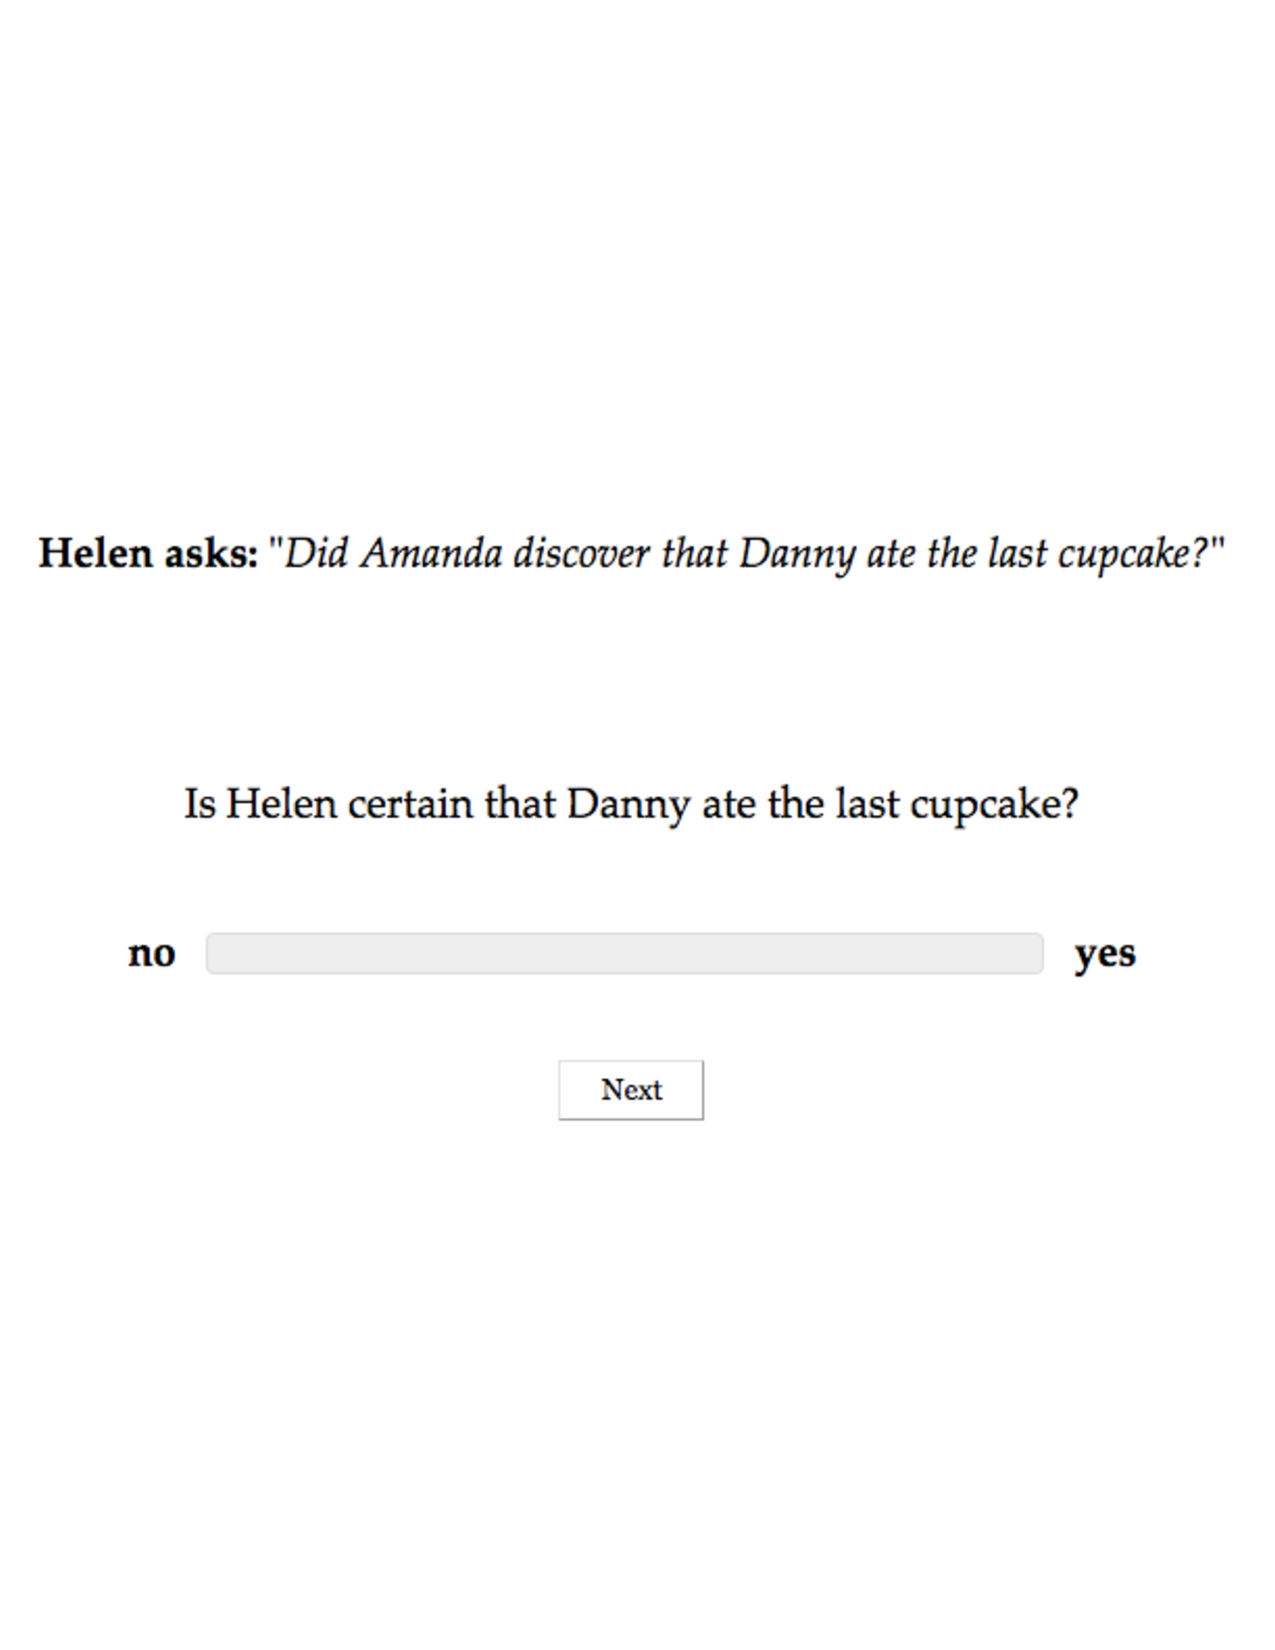
\includegraphics[width=10cm]{figures/trial-exp1}}
\end{center}
\caption{A sample trial in Experiment 1}\label{fig-trial-exp1}
\end{figure}

After completing the experiment, participants filled out a short, optional survey about their age, their gender, their native language(s) and, if English is their native language, whether they are a speaker of American English (as opposed to, e.g., Australian or Indian English). To encourage them to respond truthfully, participants were told that they would be paid no matter what answers they gave in the survey.

\paragraph{Data exclusion}
Prior to analysis, the data from XX participants who did not self-identify as native speakers of American English were excluded. For the remaining XX participants, we inspected their responses to the 6 control stimuli, for which we expected low responses because the main clause content is not expected to project from these questions. The response means of XX participants were more than XX standard deviations above the group mean of .XX for the control polar question stimuli. Closer inspection revealed that these participants' responses to the control stimuli were systematically higher or lower, suggesting that these participants did not attend to the task or interpreted the task differently. The data from these XX participants were also excluded, leaving data from XX participants (ages XX-XX; median: XX; XX female, XX male).

\subsection{Results}

The projectivity of the content of the clausal complement of the 20 clause-embedding predicates can be seen in Figure \ref{f-projectivity}: {\bf discuss details based on actual findings}.

\begin{figure}[H]
\centering

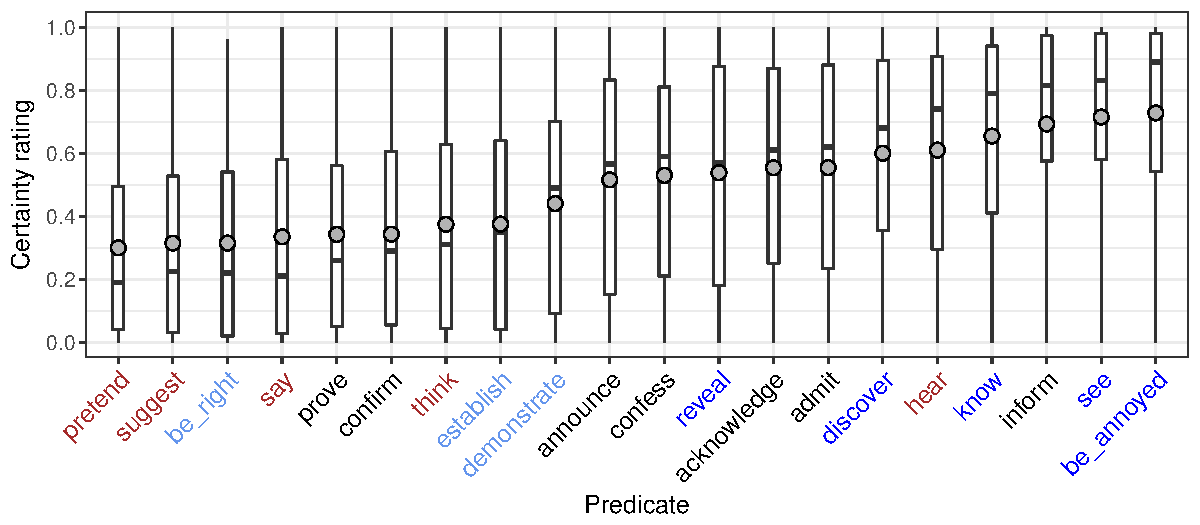
\includegraphics[width=.8\paperwidth]{../results/3-projectivity/graphs/boxplot-projectivity-factH}
%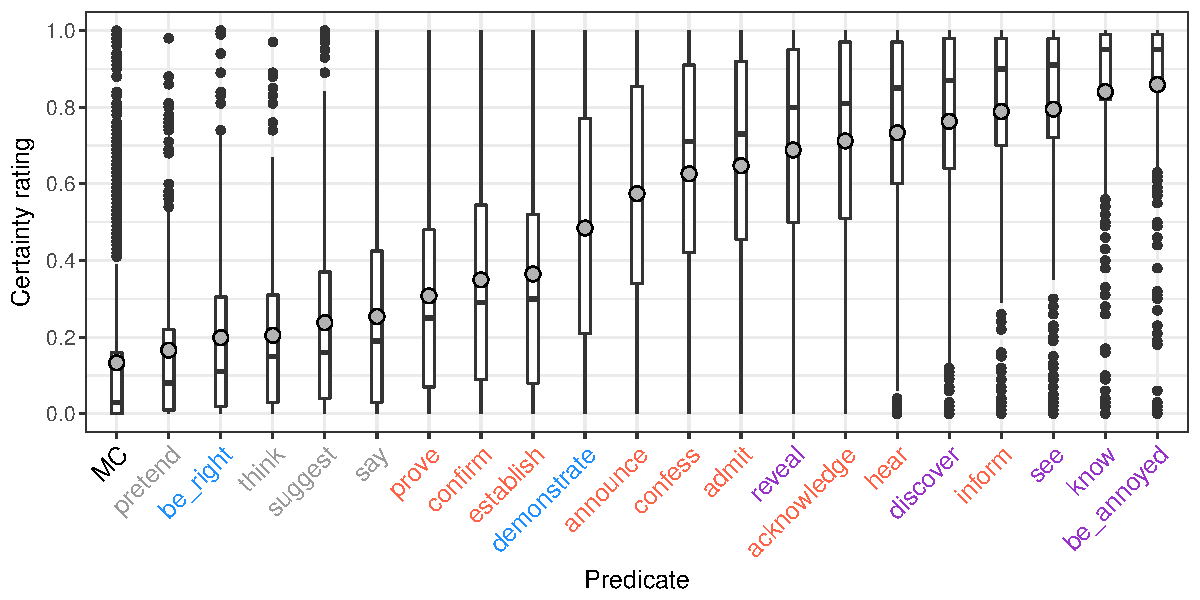
\includegraphics[width=.8\paperwidth]{../results/5-projectivity-2/graphs/boxplot-projectivity}

\caption{Box plot of certainty ratings by predicate, collapsing across complements and proper name subjects. Grey dots indicate means and notches indicate medians. `MC' abbreviates main clause. Error bars indicate 95\% confidence intervals. `Factive' predicates are given in darker blue, `veridical non-factive' ones in lighter blue, `non-factive' ones in brown and `apparently factive' ones in black.}
\label{f-projectivity}
\end{figure}

To determine which clause-embedding predicates differed from each other in the projectivity of the content of the clausal complement, we conducted post hoc pairwise comparisons using Tukey's method (allowing for by-participant variability), using the \verb|lsmeans| package \citep{tukey} in R \citep{r}. P-values for each pair of predicates are displayed in Table \ref{t-pairwise-proj}. {\bf discuss based on actual findings}

\begin{table}[H]
\setlength\tabcolsep{3pt}

\centering
\small

\begin{tabular}{l l l l l l l l l l l l l l l l l l l l }
\toprule

 &   \rot{\color{brown}{\em pretend}\color{black}} & \rot{\color{blue}{\em be right}\color{black}} & \rot{\color{brown}{\em suggest}\color{black}} &  \rot{\color{brown}{\em say}\color{black}} &  \rot{\color{black}{\em prove}\color{black}} & \rot{\color{brown}{\em think}\color{black}} & \rot{{\em confirm}} & \rot{\color{blue}{\em establish}\color{black}} & \rot{\color{black}{\em demonstrate}\color{black}} & \rot{{\em announce}} & \rot{{\em confess}} & \rot{\color{blue}{\em reveal}\color{black}} & \rot{\color{black}{\em admit}\color{black}}  & \rot{{\em acknowledge}}  & \rot{\color{blue}{\em discover}\color{black}}  & \rot{\color{brown}{\em hear}\color{black}} & \rot{\color{blue}{\em see}\color{black}}  & \rot{\color{black}{\em inform}\color{black}}  & \rot{\color{blue}{\em know}\color{black}}  \\

\midrule
%\color{brown}{\em think}\color{black}		& -- & - & - & - & - & - & - & - & - & - & - & - & - & - & - & - & - & - & - \\
\color{blue}{\em be right}\color{black}		& n.s. & - & - & - & - & - & - & - & - & - & - & - & - & - & - & - & - & - & - \\
\color{brown}{\em suggest}\color{black}			& n.s. & n.s. & - & - & - & - & - & - & - & - & - & - & - & - & - & - & - & - & - \\
\color{brown}{\em say}	\color{black}		& n.s. & n.s. & n.s. & - & - & - & - & - & - & - & - & - & - & - & - & - & - & - & - \\
\color{black}{\em prove}\color{black}		& n.s. & n.s. & n.s. & n.s. & - & - & - & - & - & - & - & - & - & - & - & - & - & - & - \\
\color{brown}{\em think}\color{black}		& n.s. & n.s. & n.s. & n.s. & n.s. & - & - & - & - & - & - & - & - & - & - & - & - & - & - \\
\color{black}{\em confirm}\color{black}		& n.s. & n.s. & n.s. & n.s. & n.s. & n.s. & - & - & - & - & - & - & - & - & - & - & - & - & - \\
\color{blue}{\em establish}\color{black}		& n.s. & n.s. & n.s. & n.s. & n.s. & n.s & n.s. & - & - & - & - & - & - & - & - & - & - & - & - \\
\color{black}{\em demonstrate}\color{black}		& *** & *** & ** & ** & * & . & n.s. & n.s. & - & - & - & - & - & - & - & - & - & - & - \\
\color{black}{\em announce}\color{black}		& *** & *** & *** & *** & *** & *** & ** & ** & n.s. & - & - & - & - & - & - & - & - & - & - \\
\color{black}{\em confess}\color{black}	& *** & *** & *** & *** & *** & *** & *** & *** & n.s. & n.s. & - & - & - & - & - & - & - & - & - \\
\color{blue}{\em reveal}\color{black}			& *** & *** & *** & *** & *** & *** & *** & *** & n.s. & n.s. & n.s. & - & - & - & - & - & - & - & - \\
\color{black}{\em admit}\color{black}		& *** & *** & *** & *** & *** & *** & *** & *** & . & n.s. & n.s. &  ns & - & - & - & - & - & - & - \\
\color{black}{\em acknowledge}\color{black}	& *** & *** & *** & *** & *** & *** & *** & *** & ** & n.s. & n.s. & n.s. & n.s. & - & - & - & - & - & - \\
\color{blue}{\em discover}\color{black}		& *** & *** & *** & *** & *** & *** & *** & *** & *** & * & . & n.s. & n.s. & n.s. & - & - & - & - & - \\
\color{brown}{\em hear}\color{black}		& *** & *** & *** & *** & *** & *** & *** & *** & *** & ** & * & n.s. & n.s. & n.s. & n.s. & - & - & - & - \\
\color{blue}{\em see}\color{black}			& *** & *** & *** & *** & *** & *** & *** & *** & *** & *** & ** & ** & * & n.s. & n.s. & n.s. & - & - & - \\
\color{black}{\em inform}\color{black}			& *** & *** & *** & *** & *** & *** & *** & *** & *** & *** & *** & ** & ** & * & n.s. & n.s. & n.s. & - & - \\
\color{blue}{\em know}\color{black}			& *** & *** & *** & *** & *** & *** & *** & *** & *** & *** & *** & *** & *** & ** & . & . & n.s. & n.s. & -  \\
\color{blue}{\em be annoyed}\color{black}		& *** & *** & *** & *** & *** & *** & *** & *** & ***  & ***  & *** & *** & *** & *** & * & * & n.s. & n.s. & ns  \\

\bottomrule
\end{tabular}
\caption{P-values associated with pairwise comparison of certainty ratings of predicate using Tukey's method. `***' indicates significance at .0001, `**' at .01, `*' at .05, `.' marginal significance at .1, and `n.s' indicates no significant difference in means. `Factive' predicates are given in darker blue, `veridical non-factive' ones in lighter blue, `non-factive' ones in brown and `apparently factive' ones in black.}\label{t-pairwise-proj}
\end{table}

{\bf Compare to findings of \citealt{tbd-variability} for {\em be annoyed, know, see, discover, establish, confess, demonstrate}}

\subsection{Discussion}

\begin{itemize}

\item Replicating \citealt{tbd-variability}, we observe variability in projectivity.

\item Overall: `factive' more projective than `veridical non-factive', `non-factive' and `apparently factive' 

\item `apparently factive' predicates also projective

\item where to draw the line between `projective' and `not projective'? unclear. so if people want to categorize, it needs to be based on veridicality.

\end{itemize}

\section{Experiment 2: Entailment}\label{s3}

The two experiments described in this section were designed explore whether the content of the clausal complement of the 20 clause-embedding predicates is an entailment, i.e., whether a positive matrix sentence of the form `NP P S' (with P a predicate) entails the clausal complement S. 

The entailment relation between sentences $A$ and $B$ is defined such that $A$ entails $B$ if and only if any world in which $A$ is true is also a world in which $B$ is true. Whether a natural language sentence $A$ entails another sentence $B$ cannot be diagnosed directly because it is impossible to verify that all worlds in which $A$ is true are also worlds in which $B$ is true. Linguists therefore rely on diagnostics that are taken to provide indirect evidence for an entailment relationship. Two standard diagnostics, referred to here as the `inference diagnostic' and the `contradictoriness diagnostic', are given in (\ref{diag}): 

\begin{exe}
\ex\label{diag} \citealt[\S3.1]{ccmg90}
\begin{xlist}
\ex  Inference diagnostic \\ $A$ entails $B$ if and only if, if $A$ is true, then the truth of $B$ definitely follows. 

\ex  Contradictoriness diagnostic \\ $A$ entails $B$ if and only if sentences of the form {\em A and not B} are contradictory. 

\end{xlist}
\end{exe}
These two diagnostics for entailment are applied in Exps.~1a and 1b to positive matrix sentences with the 20 clause-embedding predicates, to explore whether the content of the clausal complement of the 20 predicates is an entailment. We present the findings of the two experiments in sections \ref{s31} and \ref{s32}, and then discuss them together in section \ref{s33}.

\subsection{Experiment 2a: Inference diagnostic}\label{s31}

This experiment explored whether the content of the clausal complement of the 20 clause-embedding predicates is an entailment based on the inference diagnostic for entailment in (\ref{diag}a). Specifically, the experiment investigated the strength of the inference from true sentences with the 20 clause-embedding predicates to the content of the clausal complement. Gradient inference ratings were collected.


\subsubsection{Methods}

\paragraph{Participants} 300 participants with U.S.\ IP addresses and at least 99\% of previous HITs approved were recruited on Amazon's Mechanical Turk platform (ages: 19-69, median: 36; 152 female, 148 male). They were paid 75 cents for participating in the experiment.

\paragraph{Materials} The target stimuli were 400 matrix sentences that consisted of the 400 predicate-clause combinations and a random proper name subject whose gender differed from the gender of the proper name subject of the embedded clause. As illustrated in the sample stimuli in (\ref{stims2}), these matrix sentences were presented to participants as true statements. For each of the 400 target stimuli, the inference that was tested was the inference to the content of the clausal complement, for instance, to the proposition that Danny ate the last cupcake in (\ref{stims2}a) and to the proposition that Emma studied on Saturday morning in (\ref{stims2}b).

\begin{exe}
\ex\label{stims2}
\begin{xlist}
\ex {\bf What is true:} Melissa knows that Danny ate the last cupcake.
%\\ Does it follow that Danny ate the last cupcake?
\ex {\bf What is true:} Jerry pretended that Emma studied on Saturday morning.
%\\ Does it follow that Emma studied on Saturday morning?
\end{xlist}
\end{exe}

The experiment also included eight control stimuli, which were used to assess whether participants attended to the task and whether they interpreted the task correctly. For the four control stimuli in (\ref{control-good2}), the tested inferences are lexical entailment of the true statements: for instance, that Frederick solved the problem is a lexical entailment of the true statement that Frederick managed to solve the problem. We hypothesized that the inference ratings for these four control stimuli are at ceiling. In contrast, the inferences tested with the four control stimuli in (\ref{control-bad2}) definitely do not follow from these true statements: in (\ref{control-bad2}a), that Dana wears a wig does not follow from Dana watching a movie last night, and the proposition that Madison closed the window is the negation of what actually follows from the true statement in (\ref{control-bad2}c). We hypothesized that the inference ratings for these four control stimuli are at floor.

\begin{exe}
\ex\label{control-good2}
\begin{xlist}
\ex {\bf What is true:} Zack bought himself a car this morning. (Tested inference: Zack owns a car.)
\ex {\bf What is true:} Tara broke the window with a bat. (Tested inference: The window broke.)
\ex {\bf What is true:} Frederick managed to solve the problem. (Tested inference: Frederick solved the problem.)
\ex {\bf What is true:} Vanessa happened to look into the mirror. (Tested inference: Vanessa looked into the mirror.)
\end{xlist}
\ex\label{control-bad2}
\begin{xlist}
\ex {\bf What is true:} Dana watched a movie last night. (Tested inference: Dana wears a wig.)
\ex {\bf What is true:} Hendrick is renting an apartment. (Tested inference: The apartment has a balcony.)
\ex {\bf What is true:} Madison was unsuccessful in closing the window. (Tested inference:  Madison closed the window.)
\ex {\bf What is true:} Sebastian failed the exam. (Tested inference: Sebastian did really well on the exam.)
\end{xlist}
\end{exe}

Each participant saw a random set of 28 stimuli: each set contained one target stimulus for each of the 20 predicates (each with a unique complement clause) and the same 8 control stimuli. Trial order was randomized.

\paragraph{Procedure} Participants were told that they would read true statements and be asked to assess whether a second statement follows from the first, true statement. On each trial, participants read the true statement and were asked to respond to the question {\em Does it follow that\ldots} where the complement clause was a sentence that realized the inference to be tested.  Participants gave their responses on sliding scale from `definitely doesn't follow' (coded as 0) to `definitely follows ' (coded as 1), as shown in Figure \ref{f-trial-exp3}.

\begin{figure}[H]
\begin{center}
\fbox{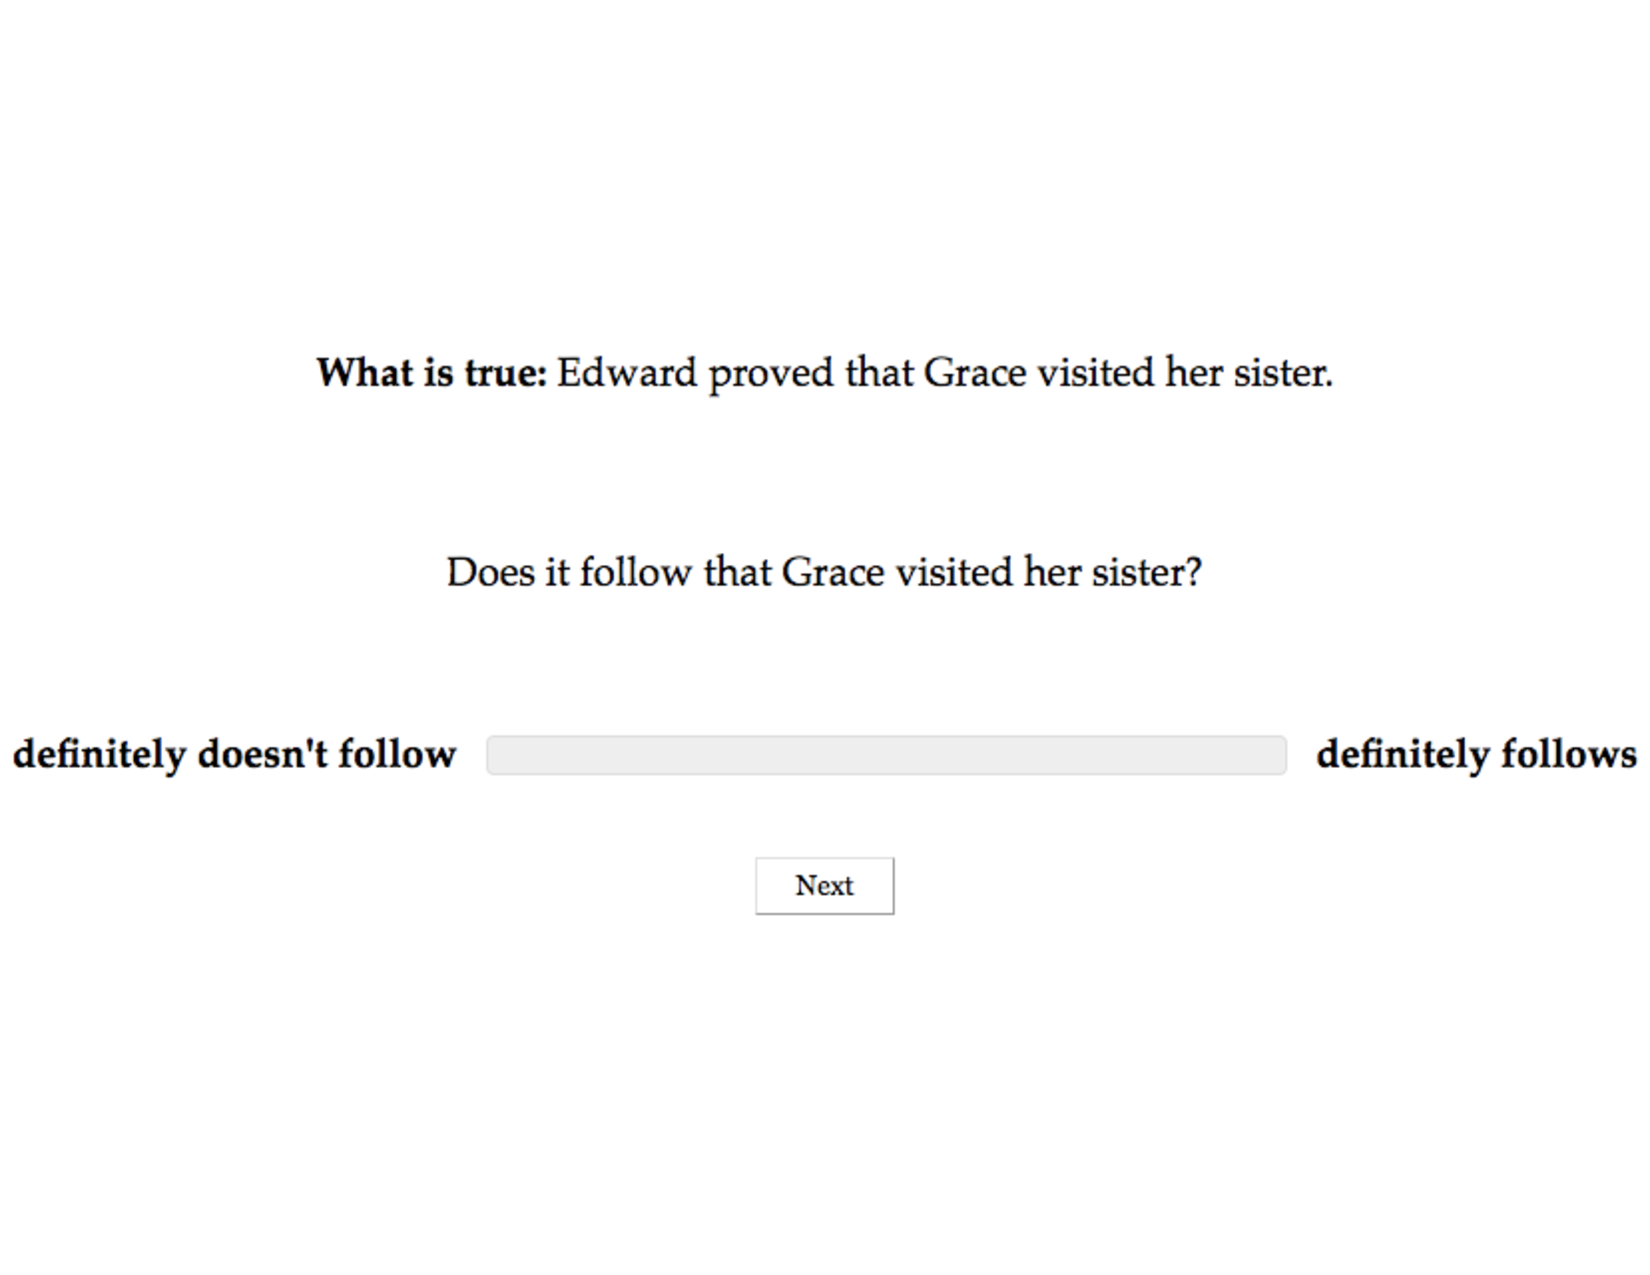
\includegraphics[width=11cm]{figures/inference-trial}}
\end{center}
\caption{A sample trial in Experiment 2a}\label{f-trial-exp3}
\end{figure}

To familiarize participants with the task, they first completed the two familiarization stimuli in (\ref{train2}), where the tested inference was the content of the clausal complement. Participants who rated (\ref{train2}a) in the lower half of the sliding scale or (\ref{train2}b) in the upper half of the sliding scale were given an explanation for why their answer was wrong. Participants could only advance to the 28 stimuli if they gave a plausible rating to the two training stimuli, i.e., a rating in the upper half of the sliding scale for (\ref{train2}a) and in the lower half for (\ref{train2}b).

\begin{exe}
\ex\label{train2}
\begin{xlist}
\ex {\bf What is true:} Drew is correct that Patty lives in Canada. 

\ex {\bf What is true}: Drew believes that Patty lives in Canada.
\end{xlist}
\end{exe}

After responding to the 28 stimuli, participants filled out a short, optional survey about their age, their gender, their native language(s) and, if English is their native language, whether they are a speaker of American English (as opposed to, e.g., Australian or Indian English). To encourage them to respond truthfully, participants were told that they would be paid no matter what answers they gave in the survey.

\paragraph{Data exclusion}
Prior to analysis, the data from 14 participants who did not self-identify as native speakers of American English were excluded. For the remaining 286 participants, we inspected their responses to the 8 control stimuli. The group means for the four control stimuli in (\ref{control-good2}) where the inference was hypothesized to follow was .94 and the group mean for the four control stimuli in (\ref{control-bad2}) where the inference was hypothesized to not follow was .05. These group means suggest that, overall, participants attended to and understood the task. The response means of 7 participants were more than 3 standard deviations below the group mean for the control stimuli in (\ref{control-good2}) or below the group mean for the control stimuli in (\ref{control-bad2}). Closer inspection revealed that these participants' responses to the control stimuli were systematically lower or higher, suggesting that these participants did not attend to the task or interpreted the task differently. The data from these 7 participants were also excluded (new group means: .95 and .04, respectively), leaving data from 279 participants (ages 19-69; median: 36; 142 female, 137 male).

\subsubsection{Results}

We expect predicates for which the content of the clausal complement is an entailment to receive inference ratings that are at ceiling. The box plot in Figure \ref{f-veridicality-predicate2} shows the participants' raw inference ratings by predicate, collapsing over the 20 complement clauses that each predicate was paired with: `factive' predicates are given in darker blue, `veridical non-factive' predicates in lighter blue, `non-factive' predicates in brown and `apparently factive' predicates in black. (This color scheme is used throughout the remainder of the paper.) The mean inference ratings of several predicates were at or close to ceiling, namely {\em prove} (.95), {\em be right} (.95), {\em see} (.94), {\em discover} (.94), {\em know} (.93), {\em be annoyed} (.92), {\em establish} (.90), {\em admit} (.90), {\em acknowledge} (.90), {\em reveal} (.90) and {\em confess} (.88). This finding suggests that participants took the truth of the content of the clausal complement of these predicates to (mostly) follow from the true statements. However, the larger box and longer whisker length for {\em reveal} already suggests that participants did not take the content of the clausal complement of this purported `factive' predicate to strongly follow from true statements with this predicate. The same holds for the purported `veridical non-factive' predicate {\em demonstrate}, whose mean inference rating was not at ceiling (.84). The `non-factive' predicates received the lowest ratings overall, as expected given the assumption that the content of the clausal complement of these predicates is not an entailment.

%          verb      Mean       YMin      YMax
%1  acknowledge 0.8980287 0.87993817 0.9159525
%2        admit 0.8984946 0.88035663 0.9165950
%3     announce 0.8034409 0.77417742 0.8306201
%4   be_annoyed 0.9150896 0.89709409 0.9314023
%5     be_right 0.9472043 0.93537455 0.9581362
%6      confess 0.8837993 0.86551523 0.9022661
%7      confirm 0.9361290 0.92328853 0.9485726
%8  demonstrate 0.8428674 0.81867204 0.8683889
%9     discover 0.9394624 0.92898835 0.9494991
%10   establish 0.8989247 0.88118100 0.9168486
%11        hear 0.4996057 0.46280108 0.5363100
%12      inform 0.8301434 0.80379301 0.8570609
%13        know 0.9251613 0.91092563 0.9387849
%14     pretend 0.1219713 0.09496774 0.1505968
%15       prove 0.9492832 0.93799194 0.9594292
%16      reveal 0.8963082 0.87770520 0.9145878
%17         say 0.6786022 0.64214785 0.7137796
%18         see 0.9426523 0.93217921 0.9526900
%19     suggest 0.3413262 0.30690950 0.3740600
%20       think 0.3138351 0.28154032 0.3453790

\begin{figure}[h!]
\centering

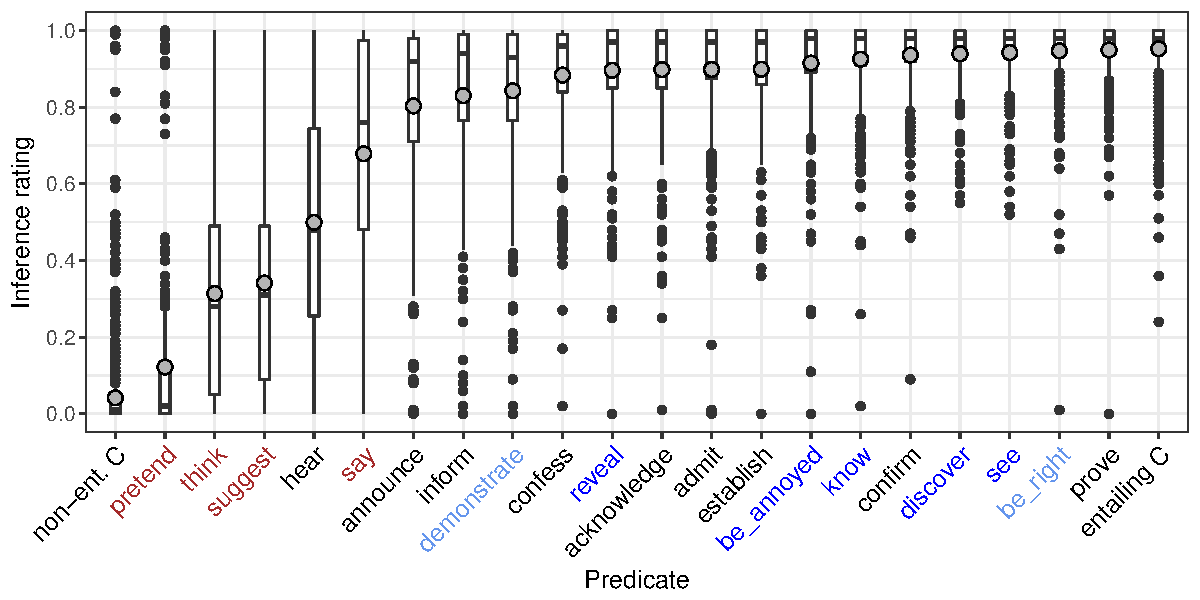
\includegraphics[width=.75\paperwidth]{../results/4-veridicality3/graphs/boxplot-inference}

\caption{Box plot of inference ratings by predicate, collapsing across complement clauses. Grey dots indicate means and notches indicate medians. Non-entailing predicates are given in brown, entailing predicates in blue, and apparently-entailing predicates are given in black.}
\label{f-veridicality-predicate2}
\end{figure}

To determine which predicates differed from each other by the strength of the inference to the content of the clausal complement, we conducted post hoc pairwise comparisons using Tukey's method (allowing for by-participant variability), using the \verb|lsmeans| package \citep{tukey} in R \citep{r}. P-values for each pair of predicates are displayed in Table \ref{t-pairwise2}. These results suggest no difference in the strength of the inference to the content of the clausal complement of the `apparently factive' predicates {\em prove, confirm, admit} and {\em acknowledge}, the `veridical non-factive' predicates {\em be right} and {\em establish}, and the `factive' predicates {\em see, discover, know} and {\em be annoyed}. However, not all `factive' and `veridical non-factive' predicates received high inference ratings: ratings for the `factive' predicate {\em reveal} were significantly lower than for the `apparently factive' predicate {\em prove}, and ratings for the `veridical non-factive' predicate {\em demonstrate} were significantly lower than for the `apparently factive' predicates {\em prove, confirm, admit} and {\em acknowledge}, for the `veridical non-factive' predicates {\em be right} and {\em establish}, and for the `factive' predicates {\em see} and {\em discover}. 

\begin{table}[h!]
\setlength\tabcolsep{3pt}

\centering
\small

\begin{tabular}{l l l l l l l l l l l l l l l l l l l l }
\toprule

 &   \rot{\color{brown}{\em pretend}\color{black}} & \rot{\color{brown}{\em think}\color{black}} & \rot{\color{brown}{\em suggest}\color{black}} &  \rot{\color{brown}{\em hear}\color{black}} &  \rot{\color{brown}{\em say}\color{black}} & \rot{{\em announce}} & \rot{{\em inform}} & \rot{\color{airforceblue}{\em demonstrate}\color{black}} & \rot{\color{black}{\em confess}\color{black}} & \rot{\color{blue}{\em reveal}\color{black}} & \rot{{\em acknowledge}} & \rot{{\em admit}} & \rot{\color{airforceblue}{\em establish}\color{black}}  & \rot{\color{blue}{\em be annoyed}\color{black}}  & \rot{\color{blue}{\em know}\color{black}}  & \rot{\color{black}{\em confirm}\color{black}} & \rot{\color{blue}{\em discover}\color{black}}  & \rot{\color{blue}{\em see}\color{black}}  & \rot{\color{airforceblue}{\em be right}\color{black}} \\
\midrule

\color{brown}{\em think}\color{black}		& *** & - & - & - & - & - & - & - & - & - & - & - & - & - & - & - & - & - & - \\
\color{brown}{\em suggest}\color{black}			& *** & n.s. & - & - & - & - & - & - & - & - & - & - & - & - & - & - & - & - & - \\
\color{brown}{\em hear}	\color{black}		& *** & *** & *** & - & - & - & - & - & - & - & - & - & - & - & - & - & - & - & - \\
\color{brown}{\em say}\color{black}		& *** & *** & *** & *** & - & - & - & - & - & - & - & - & - & - & - & - & - & - & - \\
\color{black}{\em announce}\color{black}		& *** & *** & *** & *** & *** & - & - & - & - & - & - & - & - & - & - & - & - & - & - \\
\color{black}{\em inform}\color{black}		& *** & *** & *** & *** & *** & n.s. & - & - & - & - & - & - & - & - & - & - & - & - & - \\
\color{airforceblue}{\em demonstrate}\color{black}		& *** & *** & *** & *** & *** & n.s. & n.s. & - & - & - & - & - & - & - & - & - & - & - & - \\
\color{black}{\em confess}\color{black}		& *** & *** & *** & *** & *** & *** & * & n.s. & - & - & - & - & - & - & - & - & - & - & - \\
\color{blue}{\em reveal}\color{black}		& *** & *** & *** & *** & *** & *** & ** & * & n.s. & - & - & - & - & - & - & - & - & - & - \\
\color{black}{\em acknowledge}\color{black}	& *** & *** & *** & *** & *** & *** & ** & * & n.s. & n.s. & - & - & - & - & - & - & - & - & - \\
\color{black}{\em admit}\color{black}			& *** & *** & *** & *** & *** & *** & ** & * & n.s. & n.s. & n.s. & - & - & - & - & - & - & - & - \\
\color{airforceblue}{\em establish}\color{black}		& *** & *** & *** & *** & *** & *** & ** & * & n.s. & n.s. & n.s. &  ns & - & - & - & - & - & - & - \\
\color{blue}{\em be annoyed}\color{black}	& *** & *** & *** & *** & *** & *** & *** & ** & n.s. & n.s. & n.s. & n.s. & n.s. & - & - & - & - & - & - \\
\color{blue}{\em know}\color{black}		& *** & *** & *** & *** & *** & *** & *** & *** & n.s. & n.s. & n.s. & n.s. & n.s. & n.s. & - & - & - & - & - \\
\color{black}{\em confirm}\color{black}		& *** & *** & *** & *** & *** & *** & *** & *** & . & n.s. & n.s. & n.s. & n.s. & n.s. & n.s. & - & - & - & - \\
\color{blue}{\em discover}\color{black}			& *** & *** & *** & *** & *** & *** & *** & *** & * & n.s. & n.s. & n.s. & n.s. & n.s. & n.s. & n.s. & - & - & - \\
\color{blue}{\em see}\color{black}			& *** & *** & *** & *** & *** & *** & *** & *** & * & n.s. & n.s. & n.s. & n.s. & n.s. & n.s. & n.s. & n.s. & - & - \\
\color{airforceblue}{\em be right}\color{black}			& *** & *** & *** & *** & *** & *** & *** & *** & * & . & n.s. & n.s. & n.s. & n.s. & n.s. & n.s. & n.s. & n.s. & -  \\
\color{black}{\em prove}\color{black}		& *** & *** & *** & *** & *** & *** & *** & *** & *  & *  & . & . & . & n.s. & n.s. & n.s. & n.s. & n.s. & n.s.  \\

\bottomrule
\end{tabular}
\caption{P-values associated with pairwise comparison of inference ratings of predicates using Tukey's method. `***' indicates significance at .0001, `**' at .01, `*' at .05, `.' marginal significance at .1, and `n.s.' indicates no significant difference in means. `Factive' predicates are given in darker blue, `veridical non-factive' ones in lighter blue, `non-factive' ones in brown and `apparently factive' ones in black.}\label{t-pairwise2}
\end{table}

In sum, these results support an analysis of the clausal complement of {\em prove, be right, see, discover, confirm, know, be annoyed, establish, admit} and {\em acknowledge} as an entailment. These findings do not, however, support the assumption that the content of the clausal complement of {\em reveal} and {\em demonstrate} is an entailment. Consequently, the set of `factive' and `veridical non-factive' predicates under investigation does not emerge from the inference diagnostic as a natural class of predicates whose clausal complement is an entailment. 

\subsection{Experiment 2b: Is {\em A but not B} contradictory?}\label{s32}

This experiment explored whether the content of the clausal complement of the 20 clause-embedding predicates is an entailment based on the contradictoriness diagnostic for entailment in (\ref{diag}b). Specifically, the experiment investigated the contradictoriness of utterances of positive matrix sentences with the 20 clause-embedding predicates that were followed by a denial of the content of the clausal complement. Gradient contradictoriness ratings were collected.

\subsubsection{Methods}

\paragraph{Participants} 300 participants with U.S.\ IP addresses and at least 99\% of previous HITs approved were recruited on Amazon's Mechanical Turk platform (ages: 18-72, median: 35; 137 female, 162 male, 1 other). They were paid 75 cents for participating in the experiment.

\paragraph{Materials} The target stimuli consisted of the 400 predicate-clause combinations and a random proper name subject (as in Exp.~1a) followed by a {\em but-}clause that denied the truth of the content of the clausal complement. As shown in ({\ref{stims}), the target stimuli were presented to participants as utterances by named speakers. The proper names that realized the speakers, the subjects of the 20 predicates or that occurred in the complement clauses were all unique. The gender of the proper name subject of the predicate was distinct from the gender of the proper name in the complement clause, to ensure that the pronoun in elliptical {\em but-}clause unambiguously referred to the individual referred to in the complement clause of the predicate.

\begin{exe}
\ex\label{stims}
\begin{xlist}
\ex {\bf Christopher:} {\em ``Melissa knows that Danny ate the last cupcake, but he didn't.''}
\ex {\bf Susan:} {\em ``Jerry pretended that Emma studied on Saturday morning, but she didn't.}
\end{xlist}
\end{exe}

The experiment also included eight control stimuli, which were used to assess whether participants were attending to the task. (They were also presented to the participants as utterances by named speakers.) The four control stimuli in (\ref{control-good}) were hypothesized to be non-contradictory, and the four control stimuli in (\ref{control-bad}) were hypothesized to be contradictory.

\begin{exe}
\ex\label{control-good}
\begin{xlist}
\ex Zack believes that I'm married, but I'm actually single.
\ex Tara wants me to cook for her and I'm a terrific cook.
\ex Frederick is both smarter and taller than I am.
\ex Vanessa is really good at math, but I'm not.
\end{xlist}
\ex\label{control-bad}
\begin{xlist}
\ex Dana has never smoked in her life and she stopped smoking recently.
\ex Hendrick's car is completely red and his car is not red.
\ex Madison laughed loudly and she didn't laugh.
\ex Sebastian lives in the USA and has never been to the USA.
\end{xlist}
\end{exe}

Each participant saw a random set of 28 stimuli: each set contained one target stimulus for each of the 20 predicates (each with a unique complement clause) and the same 8 control stimuli. Trial order was randomized.


\paragraph{Procedure.} Participants were told that they would read utterances made by a speaker and were asked to assess whether the speaker's utterance is contradictory. On each trial, participants read the speaker's utterance and then gave their response on a slider marked `definitely no' at one end (coded as 0) and `definitely yes' at the other (coded as 1), as shown in Figure \ref{f-trial-exp2}.

\begin{figure}[h!]
\begin{center}
\fbox{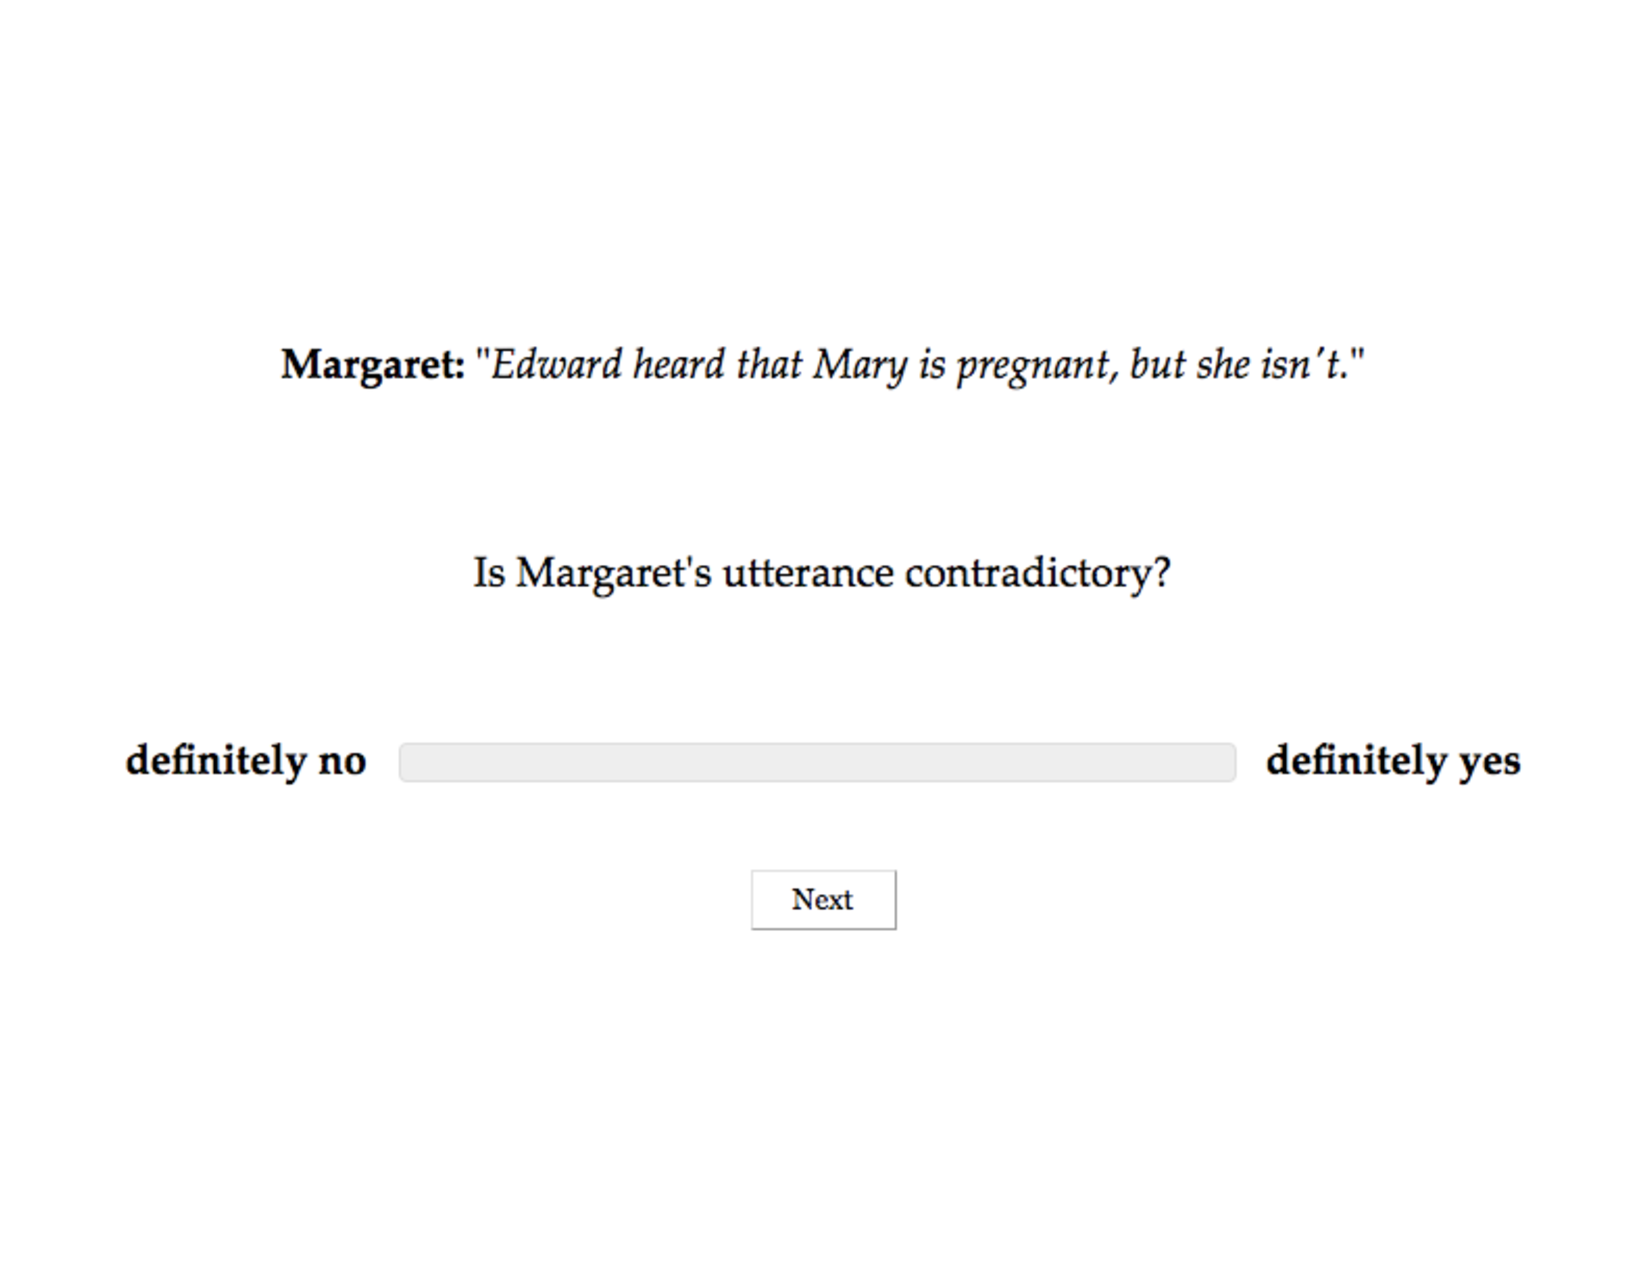
\includegraphics[width=11cm]{figures/contradictory-trial}}
\end{center}
\caption{A sample trial in Experiment 2b}\label{f-trial-exp2}
\end{figure}

To familiarize participants with the task, they first completed the two familiarization items in (\ref{train}): participants who rated (\ref{train}a) in the lower half of the scale or (\ref{train}b) in the upper half of the scale were given an explanation for why their answer was wrong. Participants could only advance to the 28 stimuli if they gave a plausible rating to the two training stimuli, i.e., a rating in the upper half of the scale for (\ref{train}b) and a rating in the lower half of the scale for (\ref{train}b).

\begin{exe}
\ex\label{train}
\begin{xlist}
\ex {\bf Bill:} Drew is aware that Patty lives in Canada, but she doesn't.

\ex {\bf Bob}: Drew thinks that Patty lives in Canada, but she doesn't.
\end{xlist}
\end{exe}

After responding to the 28 stimuli, participants filled out a short, optional survey about their age, their gender, their native language(s) and, if English is their native language, whether they are a speaker of American English (as opposed to, e.g., Australian or Indian English). To encourage them to respond truthfully, participants were told that they would be paid no matter what answers they gave in the survey.

\paragraph{Data exclusion}
Prior to analysis, the data from 19 participants who did not self-identify as native speakers of American English were excluded. For the remaining 281 participants, we inspected their responses to the 8 control stimuli: as expected, the group mean rating for the non-contradictory control stimuli in (\ref{control-good}) was at floor (.08) and the group mean rating for the contradictory control stimuli in (\ref{control-bad}) was at ceiling (.94).\footnote{The response mean of one of the non-contradictory control stimuli, (\ref{control-good}a) {\em Zack believes that I'm married, but I'm actually single}, was higher, at .17, than the response means of the remaining three non-contradictory control stimuli (which were .05 or .06). We hypothesize that some participants gave higher responses to this stimulus because the speaker can be taken to contradict Zack's belief. {\bf Either exclude participants who got this wrong from analysis, or say how the analysis doesn't change if those participants are also excluded. On the other hand, if people gave higher ratings, more sensitive to possible contradictions, that stacks the cards against us (which is good).}}  The mean ratings of 12 participants were more than 3 standard deviations above the group mean for the non-contradictory control stimuli or below the group mean for the contradictory control stimuli. Closer inspection revealed that these participants' responses to the control stimuli were systematically higher or lower, suggesting that these participants did not attend to the task or interpreted the task differently. The data from these 12 participants were also excluded (new group means: .06 and .95, respectively), leaving data from 269 participants (ages 18-72; median: 36; 128 female, 140 male, 1 other).  

\subsubsection{Results}

We expect predicates for which the content of the clausal complement is an entailment to receive contradictoriness ratings that are at ceiling. The box plot in Figure \ref{f-veridicality-predicate} shows the participants' raw contradictoriness ratings by predicate, collapsing over the 20 complement clauses that each predicate was paired with. The only predicate whose contradictoriness ratings are at ceiling is {\em be right} (mean: .93), suggesting that participants consistently took speakers to be taken to be committed to the content of the clausal complement of this predicate. In contrast, the larger box sizes, longer whisker lengths and lower mean ratings for the remaining `veridical non-factive' and `factive' predicates ({\em know} (.83), {\em see} (.81), {\em discover} (.78), {\em establish} (.72), {\em demonstrate} (.72), {\em be annoyed} (.64), {\em reveal} (.63)) suggest that participants did not consistently take speakers of target stimuli with these predicates to be committed to the truth of the content of the clausal complement. As expected, the `non-factive' predicates received the lowest ratings overall, a finding that is compatible with the assumption that the clausal complement of these predicates is not an entailment.

\begin{figure}[h!]
\centering

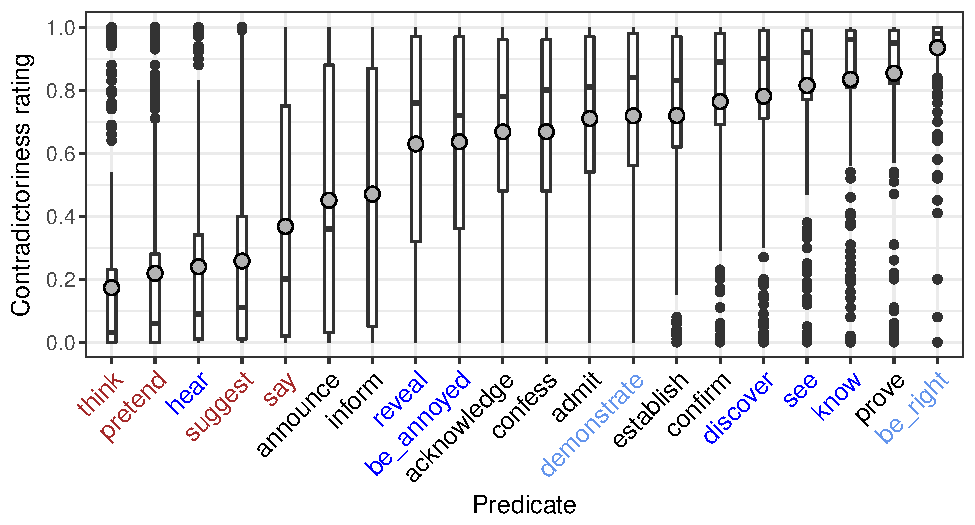
\includegraphics[width=.75\paperwidth]{../results/2-veridicality2/graphs/boxplot-veridicality}

\caption{Box plot of contradictoriness ratings by predicate, collapsing across complement clauses. Grey dots indicate means and notches indicate medians. `Factive' predicates are given in darker blue, `veridical non-factive' ones in lighter blue, `non-factive' ones in brown and `apparently factive' ones in black.}
\label{f-veridicality-predicate}
\end{figure}

To determine which predicates differed from one another in the contradictoriness ratings, we conducted post hoc pairwise comparisons using Tukey's method (allowing for by-participant variability), using the \verb|lsmeans| package \citep{tukey} in R \citep{r}. P-values for each pair of predicates are given in Table \ref{t-pairwise}. This analysis confirmed that the 5 `non-factive' predicates received significantly lower contradictoriness ratings than the 3 `veridical non-factive' and the 5 `factive' predicates. The analysis also confirmed significant differences among `factive' and `veridical non-factive' predicates. In particular, compared to the `veridical non-factive' predicate {\em be right}, the 5 `factive' predicates and the remaining 2 `veridical non-factive' predicates received significantly lower contradictoriness ratings, suggesting that speakers are taken to be less committed to the content of the clausal complement of those predicates than to that of {\em be right}. Further, both {\em demonstrate} and {\em establish} received significantly lower ratings than {\em see} and {\em know}, and both {\em be annoyed} and {\em reveal} received significantly lower ratings than {\em establish, demonstrate, discover, see} and {\em know}. 

\begin{table}[H]
\setlength\tabcolsep{3pt}

\centering
\small

\begin{tabular}{l l l l l l l l l l l l l l l l l l l l }
\toprule

 &   \rot{\color{brown}{\em think}\color{black}} & \rot{\color{brown}{\em pretend}\color{black}} & \rot{\color{brown}{\em hear}\color{black}} &  \rot{\color{brown}{\em suggest}\color{black}} &  \rot{\color{brown}{\em say}\color{black}} & \rot{{\em announce}} & \rot{{\em inform}} & \rot{\color{blue}{\em reveal}\color{black}} & \rot{\color{blue}{\em be annoyed}\color{black}} & \rot{{\em confess}} & \rot{{\em acknowledge}} & \rot{{\em admit}} & \rot{\color{airforceblue}{\em establish}\color{black}}  & \rot{\color{airforceblue}{\em demonstrate}}  & \rot{{\em confirm}}  & \rot{\color{blue}{\em discover}\color{black}} & \rot{\color{blue}{\em see}\color{black}}  & \rot{\color{blue}{\em know}\color{black}}  & \rot{{\em prove}}  \\
\midrule
%\color{brown}{\em think}\color{black}		& -- & - & - & - & - & - & - & - & - & - & - & - & - & - & - & - & - & - & - \\
\color{brown}{\em pretend}\color{black}		& n.s. & - & - & - & - & - & - & - & - & - & - & - & - & - & - & - & - & - & - \\
\color{brown}{\em hear}\color{black}			& n.s. & n.s. & - & - & - & - & - & - & - & - & - & - & - & - & - & - & - & - & - \\
\color{brown}{\em suggest}	\color{black}		& * & n.s. & n.s. & - & - & - & - & - & - & - & - & - & - & - & - & - & - & - & - \\
\color{brown}{\em say}\color{black}		& *** & *** & *** & ** & - & - & - & - & - & - & - & - & - & - & - & - & - & - & - \\
\color{black}{\em announce}\color{black}		& *** & *** & *** & *** & * & - & - & - & - & - & - & - & - & - & - & - & - & - & - \\
\color{black}{\em inform}\color{black}		& *** & *** & *** & *** & ** & n.s. & - & - & - & - & - & - & - & - & - & - & - & - & - \\
\color{blue}{\em reveal}\color{black}		& *** & *** & *** & *** & *** & *** & *** & - & - & - & - & - & - & - & - & - & - & - & - \\
\color{blue}{\em be annoyed}\color{black}		& *** & *** & *** & *** & *** & *** & *** & n.s. & - & - & - & - & - & - & - & - & - & - & - \\
\color{black}{\em confess}\color{black}		& *** & *** & *** & *** & *** & *** & *** & n.s. & n.s. & - & - & - & - & - & - & - & - & - & - \\
\color{black}{\em acknowledge}\color{black}	& *** & *** & *** & *** & *** & *** & *** & n.s. & n.s. & n.s. & - & - & - & - & - & - & - & - & - \\
\color{black}{\em admit}\color{black}			& *** & *** & *** & *** & *** & *** & *** & * & . & n.s. & n.s. & - & - & - & - & - & - & - & - \\
\color{airforceblue}{\em establish}\color{black}		& *** & *** & *** & *** & *** & *** & *** & ** & * & n.s. & n.s. &  ns & - & - & - & - & - & - & - \\
\color{airforceblue}{\em demonstrate}\color{black}	& *** & *** & *** & *** & *** & *** & *** & ** & * & n.s. & n.s. & n.s. & n.s. & - & - & - & - & - & - \\
\color{black}{\em confirm}\color{black}		& *** & *** & *** & *** & *** & *** & *** & *** & *** & ** & ** & n.s. & n.s. & n.s. & - & - & - & - & - \\
\color{blue}{\em discover}\color{black}		& *** & *** & *** & *** & *** & *** & *** & *** & *** & ** & ** & n.s. & n.s. & n.s. & n.s. & - & - & - & - \\
\color{blue}{\em see}\color{black}			& *** & *** & *** & *** & *** & *** & *** & *** & *** & *** & *** & ** & ** & ** & n.s. & n.s. & - & - & - \\
\color{blue}{\em know}\color{black}			& *** & *** & *** & *** & *** & *** & *** & *** & *** & *** & *** & *** & *** & *** & n.s. & n.s. & n.s. & - & - \\
\color{black}{\em prove}\color{black}			& *** & *** & *** & *** & *** & *** & *** & *** & *** & *** & *** & *** & *** & *** & ** & n.s. & n.s. & n.s. & -  \\
\color{airforceblue}{\em be right}\color{black}		& *** & *** & *** & *** & *** & *** & *** & *** & ***  & ***  & *** & *** & *** & *** & *** & *** & *** & ** & *  \\

\bottomrule
\end{tabular}
\caption{P-values associated with pairwise comparison of contradictoriness ratings of predicates using Tukey's method. `***' indicates significance at .0001, `**' at .01, `*' at .05, `.' marginal significance at .1, and `ns' indicates no significant difference in means. `Factive' predicates are given in darker blue, `veridical non-factive' ones in lighter blue, `non-factive' ones in brown and `apparently factive' ones in black.}\label{t-pairwise}
\end{table}

In sum, these results merely support an analysis of the clausal complement of {\em be right} as an entailment. They do not support the assumption that the content of the clausal complement of the `factive' predicates {\em know, see, discover, be annoyed} and {\em reveal} or of the `veridical non-factive' predicates {\em demonstrate} and {\em establish} is an entailment. Consequently, the set of `factive' and `veridical non-factive' predicates under investigation does not emerge from the contradictoriness diagnostic as a natural class of predicates whose clausal complement is an entailment. 

\subsection{Discussion}\label{s33}

Veridicality is one of the two properties that is assumed to distinguish `factive' from `non-factive' predicates: the content of the clausal complement of `factive' predicates is both entailed and projective, in contrast to that of `non-factive' predicates. The experiments reported on in the preceding two sections applied two standard diagnostics for entailment to the content of the clausal complement of 20 clause-embedding predicates, with the goal of identifying predicates whose clausal complement is an entailment. Table \ref{t-summary} summarizes the findings of the two experiments under the assumption that the content of the clausal complement of a clause-embedding predicate is an entailment if and only if the strength of the inference to the content is at ceiling (Exp.~2a) and a speaker who is not committed to the content is taken to contradict themselves (Exp.~2b). A checkmark `$\checkmark$' indicates that the content of the clausal complement of the clause-embedding predicate is an entailment according to the diagnostic; an `x' indicates that it is not.

\begin{table}[H]
\setlength\tabcolsep{3pt}

\centering
\small

\begin{tabular}{l c c}
\toprule
& \multicolumn{2}{c}{Entailment?} \\ 
& Exp.~2a & Exp.~2b \\ 

\midrule
\color{brown}{\em think}\color{black}		&  x &   x  \\ 
\color{brown}{\em pretend}\color{black}	&    x  &   x  \\ 
\color{brown}{\em hear}\color{black}		&    x  &   x  \\ 
\color{brown}{\em suggest}	\color{black}&    x  &   x  \\
\color{brown}{\em say}\color{black}		&    x  &   x  \\ 
\color{black}{\em announce}\color{black}	&    x  &   x  \\ 
\color{black}{\em inform}\color{black}		&    x  &   x  \\ 
\color{black}{\em confess}\color{black}		&   x  &   x  \\ 
\color{blue}{\em reveal}\color{black}		&    x  &   x  \\ 
\color{airforceblue}{\em demonstrate}\color{black} &	  x  &   x  \\ 


\multicolumn{3}{c}{\makebox[5cm]{\dashrule[black]}} \\[-\jot]

\color{black}{\em acknowledge}\color{black}	& $\checkmark$ & x \\ 
\color{black}{\em admit}\color{black}			& $\checkmark$ & x \\ 
\color{black}{\em confirm}\color{black}		&  $\checkmark$ &  x\\ 
\color{black}{\em prove}\color{black}			&  $\checkmark$ &  x\\ 


\color{blue}{\em be annoyed}\color{black}		& $\checkmark$ & x \\ 
\color{blue}{\em know}\color{black}			& $\checkmark$  &  x\\ 
\color{blue}{\em discover}\color{black}		&  $\checkmark$ &  x\\ 
\color{blue}{\em see}\color{black}			&  $\checkmark$ &  x\\ 

\color{airforceblue}{\em establish}\color{black}	& $\checkmark$ &  x\\ 

\multicolumn{3}{c}{\makebox[5cm]{\dashrule[black]}} \\[-\jot]

\color{airforceblue}{\em be right}\color{black}	& $\checkmark$  & $\checkmark$ \\ 
\bottomrule
\end{tabular}
\caption{Findings of Exps.~2a and 2b for the 20 clause-embedding predicates. `Factive' predicates are given in darker blue, `veridical non-factive' ones in lighter blue, `non-factive' ones in brown and `apparently factive' ones in black. `$\checkmark$' indicates that the content of the clausal complement of the clause-embedding predicate is an entailment according to the diagnostic; `x' indicates that it is not.}\label{t-summary}
\end{table}

As shown in Table \ref{t-summary}, the `veridical non-factive' predicate {\em be right} is the only predicate for which both experiments provide empirical support for an analysis of the clausal complement as an entailment: Exp.~2a showed that the strength of the inference to the content of the clausal complement of {\em be right} is at ceiling and Exp.~2b showed that a speaker who is not committed to the content of the clausal complement of {\em be right} is judged to be contradicting themselves. 

The findings of the two experiments are mixed for the `factive' predicates {\em see, discover, know} and {\em be annoyed} and the `veridical non-factive' predicate {\em establish}. On the one hand, Exp.~1a showed that the content of the clausal complement of the `factive' predicates {\em see, discover, know} and {\em be annoyed} and of the `veridical non-factive' predicate {\em establish} is consistently taken to follow from true statements with such predicates. This finding supports an analysis of the content of the clausal complement as an entailment. On the other hand, Exp.~1b showed that speakers who are not committed to the content of the clausal complement are not consistently taken to contradict themselves when they utter positive sentences with these predicates. This finding does not support an analysis of the clausal complement as an entailment. Crucially, these findings are identical to those for the `apparently entailing' predicates {\em prove, confirm, admit} and {\em acknowledge}: Exp.~1a showed that the content of the clausal complement is consistently taken to follow from true statements with such predicates and Exp.~1b showed that speakers who are not committed to the content of the clausal complement are not consistently taken to contradict themselves when they utter positive sentences with these predicates. In short, the experiment findings do not support a non-arbitrary division between, on the one hand, the  `factive' predicates {\em see, discover, know} and {\em be annoyed} and the `veridical non-factive' predicate {\em establish} and, on the other hand, the `apparently factive' predicates {\em prove, confirm, admit} and {\em acknowledge}.

Finally, for the `factive' predicate {\em reveal} and the `veridical non-factive' predicate {\em demonstrate}, neither of the two experiments found support for an analysis as a predicate whose clausal complement is entailed. Exp.~1a showed that the content of the clausal complement follows less strongly from true statements with these predicates than from true statements with other `factive' and `veridical non-factive' predicates, and, for {\em demonstrate}, even less strongly than for some `apparently factive' predicates. Exp.~1b showed that the speakers who are not committed to the content of the clausal complement  of {\em reveal} and {\em demonstrate} are not consistently taken to contradict themselves when they utter positive sentences with these predicates. Thus, by the findings of Exps.~2a and 2b, an analysis of the content of the clausal complement of {\em reveal} and {\em demonstrate} as an entailment is no more supported than for the `non-factive' predicates. 

In sum, the findings of the two experiments, which applied standard diagnostics for entailment to 20 clause-embedding predicates, did not finding support that the `factive' and `veridical non-factive' predicates under investigation are a natural class of predicates whose clausal complement is an entailment. We want to be very clear here that our experiments have {\bf not} shown that clause-embedding predicates cannot be classified into ones whose clausal complement is an entailment and ones whose clausal complement is not an entailment. Rather, our experiments merely show that two standard diagnostics for entailment do not provide empirical support for such a lexical classification of clause-embedding predicates. It is possible, of course, that there is a diagnostic for entailment that may be better suited to identifying a natural class of clause-embedding predicates whose clausal complements are entailments. The burden of proof, however, now lies with researchers who want to maintain such a lexical division of clause-embedding predicates. 

\section{Discussion}\label{s4}

Presuppositions have traditionally been characterized as content that is backgrounded and taken for granted (e.g., \citealt{stalnaker74,ccmg90}). In formal analyses of presuppositions, including contents of complements of clause-embedding predicates, two empirical properties of presuppositions are taken to follow from this characterization: first, presupposed content is entailed content, i.e., it necessarily follows from true statements of positive matrix sentences; second, presupposed content is projective content, i.e., the speaker is typically taken to be committed to the content even when the expression that contributes the content is embedded under an entailment-canceling operator. In particular, presupposed content is assumed to be entailed regardless of how projectivity is derived, for instance, regardless of whether projectivity arises from a requirement that presupposed content is entailed by or satisfied in the common ground (e.g., \citealt{heim83,vds92}),  is derived  from lexically-specified alternatives (e.g., \citealt{abusch10,romoli2015}), arises from a default main point mechanism (e.g., \citealt{abrusan2011,abrusan2016}) or from the question addressed by the utterance (e.g., \citealt{best-question}). 

This paper explored the presumed veridicality and projectivity of presupposed content on the basis of sentences with clause-embedding predicates: the content of the complement of `factive' predicates is analyzed as a presupposition, i.e., is taken to be both entailed and projective, and that of `non-factive' predicates is not analyzed as a presupposition. In Exps.~1 and 2, we explored the projectivity and veridicality of the content of the clausal complement of 20 clause-embedding predicates: projectivity was explored using the `certain that' diagnostic and veridicality was explored using two standard diagnostics for entailment, the inference diagnostic and the contradictoriness diagnostic. The findings of Exp.~1 showed that the content of the clausal complement of many `non-factive' predicates is projective, in some cases even more projective than that of `factive' predicates. The findings of Exps.~2  provided unanimous support for an analysis as an entailment only for the content of the clausal complement of {\em be right}. For the other `factive' and `veridical' predicates, there was either only support from the inference diagnostic (e.g., {\em know, be annoyed}) or no support at all ({\em reveal, demonstrate}) for an analysis of the content of the complement as entailed. Crucially, several `apparently factive' predicates patterned like the `factive' and `veridical' predicates. Thus, Exps.~2 did not provide support for a natural class of clause-embedding predicates for which the content of the complement can be analyzed as entailed and, consequently, no natural class of `factive' predicates emerged from Exps.~1 and 2. In short, the experiments did not find empirical support for the presumed distinction between `factive' and `non-factive' predicates.

Where do we go from here? A first possibility, already mentioned at the end of section \ref{s3}, is that there is a better diagnostic for entailment on the basis of which clause-embedding predicates for which the content of the clausal complement is an entailment can be distinguished from ones for which it is not. 

\begin{itemize}

\item What an analysis of the content of the clausal complement of `factive' predicates as a presupposition is supposed to capture is that speaker is taken to be committed to this content, whether complement clause is embedded or not. 

\item The problem is that presuppositions are defined using a binary notion of speaker commitment: either speaker is committed to truth (entailed, projects) or not necessarily committed to truth (not entailed, doesn't project).

\item So what are ways forward? 

1. Better diagnostics for entailment? Seems unlikely because our findings are consistent with previous research on veridicality. \citealt{demarneffe-etal2012}, WHITE

Our experiment findings are entirely consistent with prior research on veridicality. As discussed in \citealt{demarneffe-etal2012}, veridicality judgments are often influenced by context. 

\begin{exe}
\ex A hypothetical sentence in the New York Times: \\ United Widget said that its chairman resigned. \hfill (\citealt[302]{demarneffe-etal2012})
\end{exe}

p.302: Lexical theories of this sort provide a basis for characterizing readers? veridicality judgments, but they do not tell the whole story, because they neglect the pragmatic enrichment that is pervasive in human communication. In the lexical view, say can only be classified as non-veridical (both true and false things can be said), and yet, if a New York Times article contained the sentence United Widget said that its chairman resigned, readers would reliably infer that United Widget?s chairman resigned?the sentence is, in this context, veridical (at least to some degree) with respect to the event described by the embedded clause, with United Widget said functioning to mark the source of evidence (Simons 2007). Cognitive authority, as termed in information science (Rieh 2010), plays a crucial role in how people judge the veridicality of events. Here, the provenance of the document (the New York Times) and the source (United Widget) combine to reliably lead a reader to infer that the author intended to convey that the event really happened. Conversely, allege is lexically non-veridical, and yet this only begins to address the complex interplay of world knowledge and lexical meaning that will shape people?s inferences about the sentence FBI agents alleged in court documents today that Zazi had ad- mitted receiving weapons and explosives training from al Qaeda operatives in Pakistan last year.

p.302, footnote 2: Our use of the term ?veridicality? most closely matches that of Giannakidou (1999), where it is defined so as to be (i) relativized to particular agents or perspectives, (ii) gradable, and (iii) general enough to cover not only facts but also the commitments that arise from using certain referential expressions and aspectual morphology. The more familiar term ?factuality? seems at odds with all three of these criteria, so we avoid it.



2. Give up on the idea that presuppositions are entailments. Problematic for all kinds of analyses: lexicalist, best question, conversational implicature

3. Don't assume presuppositions, but projectivity is what should be explained. Connect explanations to lexical meanings of clause-embedding predicates. E.g., A\&H explanation for verbs of saying. Factors that matter: at-issueness, authority, prior probability. Need to investigate how much each of these properties matter.

\newpage


If, for instance, a projection analysis assumes that the content of the clausal complement to be entailed, then the analysis should only apply to  clausal complements that are, in fact, entailments. It is for this reason that \citet{schlenker10} only takes those utterances of {\em announce} to trigger a presupposition in which the content of the clausal complement is locally entailed.\footnote{\citepos{schlenker10} notion of entailment seems to be context-sensitive one, i.e., not the classical context-insensitive notion whereby a sentence $\phi$ entails a sentence $\psi$ if and only if all situations in which $\phi$ is true are situations in which $\psi$ is true. For instance, he assumes that ``in some contexts, [{\em announce}, JT\&JD] does not entail the truth of its complement; in other contexts, it entails and presupposes the truth of its complement" (p.139).} 

More drastically, \citet{anand-hacquard2014} deny that the projectivity of the content of the clausal complement of {\em announce} and {\em inform} falls into the purview of analyses of presuppositions: for them,  `non-factive' predicates merely give rise to an ``illusion of factivity'' (p.75) and an ``illusion of projection'' (p.76). They argue instead that speaker commitment to the content of the clausal complement of predicates like {\em acknowledge, admit} and {\em confirm} arises from these predicates reporting ``discourse moves which lead to the acceptance of the complement $p$ into the common ground of the reported discourse'' (p.74) and then ``[t]his acceptance of p can easily bleed into the actual common ground'' (p.75). Thus, once the content of the complement of a clause-embedding predicate is determined to not be an entailment, i.e., the predicate is `non-factive', the projectivity of the content of the clausal complement must be derived differently than for `factive' predicates.

It is uncontroversial that projectivity may derive from different sources for different kinds of content: see, for instance, \citealt{potts05} on conventional implicatures, \citealt{beaver-clark08} on the prejacent of {\em only} or \citealt{abrusan2013} on the prejacent of manner adverb utterances.  For the clause-embedding predicates, too, it is possible that the projectivity of the content of the clausal complement should be derived from different sources: for instance, along the lines of \citepos{anand-hacquard2014} proposal for `non-factive' reporting predicates and along the lines of \citealt{abusch10,abrusan2011} and \citealt{romoli2015} for `factive' predicates whose clausal complement is less highly projective. It is critical, therefore, to understand which clausal complements form a natural class. In this paper, we examine whether `factive' predicates form a natural class and, in particular, whether the veridicality and projectivity of the content of the clausal complement of `factive' predicates empirical motivates considering such predicates to form a natural class. We already saw above that projectivity is not a property that distinguishes `factive' from `non-factive' predicates. 

\end{itemize}

\section{Conclusions}\label{s5}

\appendix

\setcounter{table}{0}
\renewcommand{\thetable}{A\arabic{table}}

\setcounter{figure}{0}
\renewcommand{\thefigure}{A\arabic{figure}}

\section{20 complement clauses}\label{a-clauses}

The 20  clauses that realized the complement clauses of the 20 clause-embedding predicates in Experiments 1 and 2 are as follows:

\begin{enumerate}[leftmargin=3ex,itemsep=-2pt]

\begin{multicols}{2}

\item Mary is pregnant.
\item Josie went on vacation to France.
\item Emma studied on Saturday morning.
\item Olivia sleeps until noon.
\item Sophia got a tattoo.
\item Mia drank 2 cocktails last night.
\item Isabella ate a steak on Sunday.
\item  Emily bought a car yesterday.
\item  Grace visited her sister.
\item Zoe calculated the tip.

\columnbreak

\item  Danny ate the last cupcake.
\item  Frank got a cat.
\item  Jackson ran 10 miles.
\item  Jayden rented a car.
\item  Tony had a drink last night.
\item  Josh learned to ride a bike yesterday.
\item  Owen shoveled snow last winter.
\item  Julian dances salsa.
\item  Jon walks to work.
\item  Charley speaks Spanish.

\end{multicols}

\end{enumerate}

\section{SALT comments -- digest, then delete!}


{\bf SALT reviewer feedback / lessons}

\begin{itemize}

\item R1: very interesting study, experiment is well worth doing; what are the main theoretical implications?

\item R2: Historically (Langendoen\&Savin, Karttunen) the term "project" was applied to presuppositions, not to entailments. The terminology in this paper is confusing. There is an unstated theoretical premise of the paper is that so-called presuppositions are really just entailments and the classical projection problem should be framed in another way.

If the question is whether the content of a complement clause is interpreted as a speaker's belief, it includes cases that involve neither entailments nor presuppositions. For example, take Karttunen's one-way implicatives such as 'be able.'  [...]

discussion in Karttunen’s 2016 SALT paper under the heading Invited Inferences.

``hear'': involves another speaker, communicative intent of current speaker could be to just convey the content of the complement [connection to evidentials]

A poor choice of examples might explain the puzzling data about the discrepancy of between the two figures for the 'be right' construction. 

\item R3: hard to connect the reported experimental results with questions of semantic theory

most theories don't treat projectivity as a theoretical notion, so it strikes me as more reasonable to frame the discussion in terms of the relevant theoretical entities (presuppositions, etc.) rather than in terms of an epiphenomenal notion such as projectivity.

even if we think that it makes sense to study projectivity, why should we investigate correlations with factors such as event probability?

The authors suggest a correlation between at-issueness (which has been argued to be involved in projection) and probability, but then doesn't it make more sense to investigate at-issueness directly rather than event probability? Of course, it is conceivable that probability is easier to study and can serve as a proxy for at-issueness, but then this should be made explicit, and the choice should be accompanied with an explanation of why studying the proxy (rather than the actual entity of interest) is still meaningful.

\item R4: It is never verified in this experiment or in cited literature that the norming procedure 2 as performed with Turkers gives information that maps onto the logical-linguistic-philosophical notion of contradictoriness vs. compatibility.  This needs to be evaluated with reference to a range of sentences of different types.  The data here are compatible with the position that a contradictoriness score above 0.6 indicates that [x R p] entails p in the logical-linguistic sense, in an unqualified way.

The procedure described around (3) [task in projectivity experiment] oddly non-naturalistic, because for verbs that are really presuppositional, it results in discourses where the presupposition is not supported.

Anyway, it would be valuable to include this paper if there is space in the conference, since such issues should be discussed.

\item R5: While I’m sympathetic to the goal of understanding better how projection works, I’m not convinced that the results really tell us anything we didn’t know before.

First, the experiment gives very partial contexts, and I thus wonder whether it really tests projection or whether the task may have been a bit metalinguistic, with subjects trying to reconstruct what the expected answers were supposed to be.

are the results unexpected in any way? As for event probability, in a context with little to go by other than a potential link between the given fact and the event described by the complement, the assumption that less probable events are more at issue than more probably events seems reasonable. But we already know from the literature that at-issue-ness affects projectivity.

we already know from the literature that not all that is entailed projects (non factive veridical predicates like ‘be right’), and that not everything that projects is entailed (data in (i)) [complement of announce projects but is not entailed]. Is the goal of the study to show that this holds even with naive speakers? Is there reason to doubt the judgments reported in the existing literature? To better appreciate the contributions of this experiment, it would be useful to see what exactly is novel and unexpected and what motivates the need for an experiment.

\item R6:  It makes no sense to me to call this veridicality.  Would the author also want to say that truth itself is gradable? 

\item R7: The finding that projectivity is influenced by prior probability is (as far as I know) new and if is true more broadly, it opens new avenues of thinking on the projection problem. This is the aspect of the paper that I find the most exciting.

Though I happen to agree with the conclusion the author(s) draw(s), I think they should tread carefully. The point about part-time triggers was that they can appear factive when a rich context licenses a veridical(ish) inference. Given that (2) and (3) were presented without much surrounding context, it is unclear whether this heavily context-dependent aspect of part-time triggers was captured by the tests of the authors.

\item R8: why did you not cite Giannakidou for veridicality?!?

\end{itemize}

\section{Other stuff}


\begin{itemize}

\item Presuppositions are backgrounded info, even when they are new info:

\begin{itemize}

\item \citealt[205]{levinson83}: ``It is sufficient, as Gazdar (1979a: 105ff) notes, that what I presuppose is {\em consistent with} the propositions assumed in the context. It is interesting to note that (164) [{\em I'm sorry I'm late, my fire-engine broke down}] is probably {\bf not appropriate} in circumstances where it is not mutual knowledge that the presupposition (165) [The speaker has a fire-engine] is true...presumably because it is not consistent with the average man's beliefs that an average man owns a fire-engine (but see Prince, 1978b for some more complex explanations).''

\item \citealt[252]{simons2003}: ``This is the well known fact that a speaker need not actually believe that the presuppositions of the sentences she utters are part of the accepted background information at the time of utterance. It is quite common and natural for speakers to use presupposing sentences to inform their hearers that the presuppositions are true (or at least, that they believe so, or intend their hearers to believe so). This is particularly {\bf unproblematic} when the presupposition is uncontroversial information which is secondary to a speaker’s main point.


\citealt[899]{prince1978}: ``Why does new information occur in these logically presupposed {\em that-}clauses? [...] Their function, or at least one of their functions, is to mark a piece of information as a fact, known to some people although not yet known to the intended hearer. [...] Thus they are frequent in historical narrative, or wherever the speaker wishes to indicate that s/he does not wish to take personal responsibility for the truth or originality of the statement being made. In a sense, they are similar to hedges -- e.g., {\em It seems that, I think that, sorta} -- since both have the effect of reducing the speaker's responsibility. Hedges do this by weakening the statement, but making it into a `guess' or conjecture; {\em it-}clefts do it by strengthening the statement, by presenting it as an already known fact.''

p.903:

\begin{exe}
\ex
\begin{xlist}
\ex Given information: Information which the co\"operative speaker may assume is appropriately in the hearer's consciousness.

\item Known information: Information which the speaker represents as being factual and as already known to certain persons (often not including the hearer).

\end{xlist}
\end{exe}

``Known information, however, is less related to what one thinks of as `grammar', and less immediately relevant to speaker-hearer interaction. It is rather a choice on the part of the speaker of a particular validity-level that s/he wishes to ascribe to the utterance. Markers of this choice [...] include the {\em it-}cleft and particular word choices ({\em the fact that}, factive predicates etc.). [...] known information may also signal deference, for the same reason that hedges do: both lessen the speaker's responsibility for the statement made; they reduce the speaker's assertiveness, claims to originality -- and, therefore, role.''

\item Bolinger (1977:68): ``A factive verb implies the factuality of its complement in the mind of the hearer, not the shared knowledge of it between speaker and hearer.''

\end{itemize}

\item {\bf Motivation to look at entailment}

\begin{itemize}

\item Some theoretical analyses of presuppositions assume that some presuppositions are entailments of unembedded sentences. (As Mandy pointed out in her email, most people wouldn't assume that the ps of {\em too} is an entailment; rather, it is a constraint on felicitous use of the sentence.) The content of the complement of attitude predicates, however, is a place where the question really comes up and has come up.

\item Mandy: ``What you wind up with is the observation that be annoyed -- one of the standard presuppositional verbs -- is demonstrably more projective than other verbs, not standardly considered presuppositional, that have the same degree of veridicality, in your sense. So, a theorist might say: OK, this is great: this shows that we were *right* to treat the factive implication of be annoyed as special, and to analyze its projectivity as stemming from a special linguistic feature. The fact that in use, some sentences containing non-presuppositional verbs can give rise to parallel implications, perhaps even more strongly, doesn't mean that we shouldn't have identified this implication as linguistically special to begin with.''

\item David: ``I worry that maybe your (iii) is not the right claim to consider. The claim is: "veridicality (a gradient measure of the extent to which the clausal complement is entailed) is not a predictor of projectivity”. But here it’s unclear what “predictor” means. What you appear to test, more narrowly, is whether knowing to what extent something is veridical provides evidence of the degree to which it is projective in a linear model. But I think the most people had been assuming is that veridicality is something like a necessary condition for presupposition related projectivity, which does not imply to would be a good predictor in a linear model. Note that I say “presupposition related projectivity” because I’m not sure that the assumption has ever been explicit for conventional implicatures. But even ignoring this caveat, saying that X is a necessary condition for Y does not in any way imply that knowing X would provide evidence for Y. It tells you that knowing NOT X would provide evidence for NOT Y.''

\item David: ``Unfortunately, there isn’t agreement about  “projection” means, a situation Mandy has been trying especially hard to rectify. But I don’t think anyone had assumed that in general utterances containing propositions embedded in non-veridical contexts would never provide evidence that the speaker believed those propositions. If I ask “Did Mary tell you she’s going to be a few minutes late?”, it’s quite natural to conclude that I think Mary is going to be a few minutes late, and I don’t think many people who’ve been working on presupposition over the years would conclude their theories were wrong on that basis. I think they’d rather say that the inference was some sort of implicature, and their theories were never intended to cover it. Whether that’s a legitimate response or not is a methodological issue… I can’t see it being resolved by finding the rate of projectivity for “tell” and other verbs with non-veridical propositional complements.''

\begin{itemize}

\item Beaver 01: p.67: ``\citealt[196-198]{vds88} makes it clear that he regards the flexibility of a theory in which presuppositions do not have to be entailed as a major boon.''

\item Beaver 01: p.67: ``van der Sandt mentions emotive factives, like {\em is glad, regrets}, a class of verbs which Gazdar (1979a, pp. 122-123) argues to entail their presuppositions. Gazdar's claim runs {\em contra} to an earlier observation of Klein (1975), discussed by Gazdar, that utterances of sentences like E78 [{\em Falsely believing that he had inflicted a fatal wound, Oedipus regretted killing the stranger on the road to Thebes}] do not indicate the complement of {\em regret} to be true.''

\item Beaver 01: p.67: ``There is good reason to remain suspicious of non-entailed presuppositions, for making this move creates as many problems as it solves.'' ARGUMENTS ARE NOT OF EMPIRICAL NATURE BUT RATHER BASED ON CANCELLATION ACCOUNTS MAKING WRONG PREDICTIONS

\end{itemize}

{\bf which of these are found with {\em falsely}?}

\begin{itemize}

\item ``falsely annoyed that'': no hits

\item ``falsely annoyed NP'' HITS!


\end{itemize}

\end{itemize}


\item CCMG on presuppositions:


- p.355: A entails B: if A is true, B is true

A presupposes B: B is backgrounded and taken for granted by A

- p.355: P projecting is taken as evidence for backgroundedness and taken for granted

- p.355: A sentence can both entail and presuppose another sentence as the former notion is based on how an implication is licensed, while the latter is based on its discourse status. 

"Joan realizes that syntax deals with sentence structure" both entails and presupposes the content of the clausal complement

and again here they point to projection as a way of showing backgroundedness and taken for granted

- p.355: On the definition of entailment that we have so far, a sentence can presuppose another sentence without entailing it.

If Bill discovers that syntax is easy, he will be delighted.

presupposes syntax is easy but doesn't entail it: it ``needs'' the clausal  complement ``for felicity'' (p.356)

- p.361, (52): A sentence S presupposes a proposition p iff in any context where S has a semantic value relative to c (is true or false relative to c), p follows from the common ground of c...

- p.380: ``we have maintained that the main features of presuppositions are (a) their survival in various contexts (the P family),... and (b) their defeasibility in certain circumstances.''

p.349f.: ``the main empirical characteristics of presuppositions can be taken to be the following two: being backgrounded and being taken for granted.'' THIS DOES NOT INCLUDE BEING ENTAILED!! 

p.350: ``What the P family test essentially tests for is backgroundedness of implications: it marks out implications that are attached to S, not only when it is asserted but also when it is denied, questioned, or offered as a hypothetical assumption.''

p.352: ``The hallmark of a presupposition is that it is taken for granted in the sense that its assumed truth is a precondition for felicitous utterance of the sentence and places a kind of constraint on discourse contexts that admit the sentence for interpretation. [...] The P family test does not definitively identify presuppositions, because background status of an implied proposition is compatible with its being presented as not already assumed. If there is no suggestion of infelicity in using S in a discourse where p is clearly not taken to be part of the common ground, then S does not presuppose p even if p is backgrounded by S (as in the case of nonrestrictive relative clauses).''

SPENADER: many presuppositions are new information in discourse 


\end{itemize}

\newpage

\begin{itemize}

\item For the presupposition of semi-factive predicates people have given non-lexicalist analyses (e.g., \citealt{abrusan2011,abrusan2016,best-question}), i.e., they still assume it's a presupposition and hence belongs in the set of predicates that need to be given an explanation.

Explanations crucially rely on the content of the clausal complement being entailed.

\item Generally presuppositions are assumed to be entailed; this arises from lexicalist analyses which require p to be entailed by or satisfied in CG even in unembedded sentences.

\begin{itemize}

\item \citealt[345]{vds92}: ``Note that this is what we would expect given the intuitive notion of presupposition as information taken for granted and note also that this explains the intuition that presuppositions, unless filtered, cancelled or neutralized, are entailed by their matrix sentence.''

\item \citealt[119-123]{gazdar79a}, described in \citealt[66f.]{beaver01}: ``Gazdar (1979a, pp. 119-123) describes the inferences associated with factive verbs, definite descriptions, aspectual verbs, and clefts as being indefeasible in simple affirmative sentences. Since potential presuppositions are always defeasible in Gazdar's model, and since the only inferences which are indefeasible in his model are those associated with the asserted content, Gazdar is forced to claim that the potential presuppositions of these constructions are also entailments.''

\item Presuppositions are sometimes contrasted with “ordinary entailments” or “regular entailments”, i.e., as if they were a special sort of entailment. E.g., https://plato.stanford.edu/entries/presupposition/ or Abbott \& Horn (Where have some of the presuppositions gone?) "we will need to be careful to distinguish entailments that are presupposed from what I will call “ordinary, simple entailments”, which are not also presuppositions”; same paper: "The crucial difference, one more time, is that presuppositions are entailed by S (i.e. are part of the truth conditions of S),"

\item \citealt[139]{schlenker10}: "we obtain the pattern of inference which is characteristic of presuppositions: an entailment of the positive sentence is preserved under negation and in questions, and it gives rise to a universal inference under the quantifier no.”

\item \citealt[355]{ccmg90}: A sentence can both entail and presuppose another sentence as the former notion is based on how an implication is licensed, while the latter is based on its discourse status.
?Joan realizes that syntax deals with sentence structure? both entails and presupposes the content of the clausal complement

\citealt[354]{ccmg90}: {\em Discover} is a factive, which is to say that if $x$ discovers $p$, $p$ must be the case. 

\item \citealt{anand-hacquard2014}: p.77: ?we will adopt the pragmatic view of presupposition triggering, according to which presuppositions are lexical entailments that are backgrounded based on pragmatic principles p.71: ?Thus, under the pragmatic view of triggering, a predicate is factive because its ve- racity entailment is backgrounded, and a predicate is veridical if its veracity entailment is foregrounded.?

\citealt{anand-hacquard2014}: They also say (p.71): "One common and influential line of explanation has been to assume that both presupposed and at-issue content are, semantically speaking, entailments of a linguistic expression, but that presuppositions come about when entailments are backgrounded according to pragmatic principles."

\end{itemize}

\end{itemize}



\bibliographystyle{/Users/tonhauser.1/Library/Latex/cslipubs-natbib}
\bibliography{/Users/tonhauser.1/Documents/bibliography}

\end{document}
